\documentclass[preprint,12pt]{elsarticle}

% --- Fonts & language ---
\usepackage[T1]{fontenc}
\usepackage[utf8]{inputenc}
\usepackage{lmodern}
\usepackage[english]{babel}
\usepackage{microtype}

% --- Math ---
\usepackage{amsmath}
\usepackage{amssymb}
\usepackage{mathrsfs}

% --- Figures, tables, floats ---
\usepackage{graphicx}
\usepackage{float}
\usepackage{booktabs}   % nicer tables
\usepackage{multirow}
\usepackage{placeins}   % FloatBarrier etc.

% --- Text symbols ---
\usepackage{textcomp}
\usepackage{gensymb}

% --- Captions & subfigures (load caption before subcaption) ---
\usepackage{caption}
\usepackage{subcaption}

% --- Bibliography (load before hyperref) ---
\usepackage{natbib}

% --- Misc ---
\usepackage{url}        % optional; hyperref supersedes most of it
\usepackage{lineno}     % load after hyperref (see below)

% --- Hyperlinks ---
\usepackage[unicode,hidelinks]{hyperref}

% After \begin{document}, enable line numbers:
% \linenumbers

\journal{Nature Communications}

\begin{document}
\begin{frontmatter}

%% Title, authors and addresses
\title{Lower-Dimensional, Optimized Representations of High-Level Information in Chess Experts}

\author[inst1]{Andrea I. Costantino\corref{cor1}}
\ead{andreaivan.costantino@kuleuven.be}
\author[inst2]{Merim Bilalic}
\author[inst1]{Hans Op de Beeck}

\cortext[cor1]{Corresponding author}

\address[inst1]{Brain and Cognition, Faculty of Psychology and Educational Sciences, KU Leuven, Leuven, Belgium}
\address[inst2]{Department of Psychology, Northumbria University, Newcastle upon Tyne, UK}

\begin{abstract}
What transforms a novice into an expert? While decades of research show that expertise relies on rich, domain-specific knowledge, a precise neural account of this transformation has been missing. We lack a clear understanding of what information expert representations encode, how they are structured for efficient use, and where in the brain they reside. Here, using chess as a model system for high-level skill, we combine neuroimaging with multivariate pattern analysis to reveal three core principles of the expert brain. We show that expertise drives a shift in representational content, from low-level perceptual features to abstract, relational information. This is accompanied by a structural change, where neural codes become more compressed and geometrically optimized. Finally, we find the representational load shifts from sensory-specific cortices to domain-general frontoparietal networks. These principles define a network-code inversion that resolves a central paradox of expertise, explaining how the brain packs richer knowledge into more efficient codes for the rapid, flexible decision-making that defines mastery.
\end{abstract}

\begin{keyword}
expertise, chess, representational similarity, manifold dimensionality, fMRI, MVPA
\end{keyword}

\end{frontmatter}
\linenumbers

\newpage

\section{Introduction}  

% OPENING: Central question and domain importance
What makes a novice into an expert? This longstanding question sits at the intersection of neuroscience, cognitive science, and artificial intelligence \cite{bilalic_mechanisms_2010,ericsson2007capturing,lake2017building,mcgrath2022acquisition,ericsson1993role,anderson1982acquisition}. Across diverse domains such as mathematics~\cite{grabner_individual_2007, pesenti_mental_2001}, language~\cite{siegmund_understanding_2014,floyd_decoding_2017}, motor skills~\cite{gerloff_stimulation_1997,jancke_architecture_2009,naito_efficient_2014}, and chess [REF], extensive experience equips individuals with domain-specific knowledge, which serves as the foundation for fast, accurate, and flexible decision-making. Decades of cognitive research have established how such knowledge supports expert performance at the behavioural and computational levels. Yet, we still lack a precise account of its neural basis: specifically, \textbf{\emph{what}} information expert representations encode (the \emph{content}), \textbf{\emph{how}} that information is organized for efficient readout (the \emph{structure}), and \textbf{\emph{where}} in the brain such representations are expressed (the neural \emph{substrate}). 

% THEORETICAL FOUNDATIONS: Classical expertise research
A century of research on expertise has revealed that outstanding performance rests much more on knowledge than on raw general ability~\cite{gobet2004moves,gobet2017understanding}. Years of focused exposure tune perception and memory to a domain's recurring structure~\cite{gobet2001chunking,ericsson1993role}. Co-occurring features are compressed into chunks~\cite{chase1973perception} and richer templates~\cite{gobet1996templates} that bind surface cues to deeper relations and typical courses of action. When familiar constellations appear, they trigger these stored structures, which rapidly ``unpack'' the relevant details and predictions~\cite{chase1973perception,gobet1996templates,gobet2001chunking}, functioning like an extension of working memory~\cite{ericsson1995long}. This enables experts to grasp a situation's underlying structure while simultaneously preparing appropriate responses~\cite{boggan2012chess}. Novices, by contrast, organize by appearances and get stuck on particulars. Expert cognition is therefore qualitatively different: recognition-driven and relational, powered by compact yet flexible knowledge that supports both a quick overview and fine-grained analysis when needed~\cite{bilalic2017neuroscience,bilalic2018double}.

% NEURAL CORRELATES: Neuroimaging findings on expertise
Neuroimaging studies confirm that expertise involves a functional reorganization of neural resources toward domain-specific and memory-based processing, which enable access to knowledge for fast, accurate decisions~\cite{bilalic2017neuroscience,williams2025neural,guida2013functional}. Across domains, these systems are engaged more strongly (and often bilaterally) in experts than in novices~\cite{bilalic2018double}. The precise loci depend on stimulus type. In chess, experts preferentially recruit lateral temporal and parietal regions for object identities and functions but invoke scene/navigation systems for pattern recognition~\cite{krawczyk2011neural,bilalic_mechanisms_2010,bilalic2011takes,bilalic2012expertise,bartlett_expertise_2013,langner2019network}. Radiological expertise, with its holistic processing at its core, is characterized by ventral occipito-temporal selectivity~\cite{harley2009engagement,bilalic_revisiting_2016,kok2021holistic,ouellette2020functional}. In higher-level calculation, professional mathematicians engage a bilateral frontoparietal-temporal network~\cite{amalric2016origins,jeon2017does}, while mental calculators draw on episodic memory components in the temporal lobe~\cite{pesenti2001mental}. When computation is externalized, as with the abacus, experts rely on visuospatial and premotor simulation circuits related instrument manipulation~\cite{tanaka2002superior,hanakawa2003neural}. Finally, in motor expertise, premotor-parietal action-observation network engages earlier, enabling anticipation from kinematic cues~\cite{aglioti2008action}. 

% METHODOLOGICAL GAP: Limitations of current approaches
These studies mostly rely on univariate contrasts--highlighting regions with increased activation that do not reveal the structure or content of the encoded information. We know which regions are more active in experts, but not how they represent domain-specific knowledge. To close that gap, we move from localization to representational geometry, investigating how domain knowledge is represented. Addressing these questions requires analytical methods that go beyond behavioural measures and region-wise activation. 

% METHODOLOGICAL APPROACH: MVPA and representational analysis
Multivariate pattern analysis (MVPA)--including decoding and representational similarity analysis (RSA)--offers a powerful framework to probe the informational content and structure of neural activity~\cite{Kriegeskorte2008, Kriegeskorte2013}. These methods allow us to quantify not just whether two conditions elicit different responses, but how stimuli are internally represented and organized in representational space  \cite{bracci2023understanding, Kriegeskorte2008, contier2024distributed}. While MVPA approaches have been transformative in vision~\cite{haxby2001distributed,Kriegeskorte2008,kamitani2005decoding}, language~\cite{mitchell2008predicting,huth2016natural}, and memory research~\cite{polyn2005category,xue2010greater}, they remain underused in the study of high-level cognitive expertise.

% CURRENT STUDY: Approach and research questions
Here, we apply these methods to the domain of chess, a model system in cognitive science and artificial intelligence~\cite{Chase1973,mccarthy1990chess}, with objective performance metrics (Elo) and constrained yet ecologically valid stimuli. We combine behavioural measures with univariate fMRI, MVPA (decoding/RSA), and manifold-based dimensionality analyses to ask not only where experts and novices show different average activations, but also \textbf{what} information expert representations encode (content), \textbf{how} that information is organised for efficient readout (structure), and \textbf{where} in the brain these codes are expressed (distribution). This representational approach moves beyond localisation or activation-based accounts by characterising the internal geometry of neural codes rather than their magnitude alone.

\begin{figure}[!tp]
  \centering
  \includegraphics[width=1\textwidth]{write/figures/graphical-abstract.png}
  \caption{
    \textbf{Overview of questions, analyses, and results.}
    Chessboard stimuli in the fMRI task elicit multivoxel patterns used to answer \textbf{what} is represented, \textbf{how} it is structured, and \textbf{where} it is expressed. \textbf{Left:} Whole-brain RSA and univariate maps quantify network involvement and representational shifts (where); ROI summaries localize effects. \textbf{Right:} Voxel patterns are parcellated with coarse Glasser ROIs (colors indicate cortical families, e.g., primary visual, frontal) to perform ROI-based RSA/decoding (what) and to estimate participation ratio and test linear separability (how).}
      \label{fig:analysis_summary}
\end{figure}

% THEORETICAL CONTRIBUTION
Using this multilevel framework, we show that expert representations prioritise relational, goal-relevant information over surface features (content), are more compact yet more linearly separable while preserving fine detail (structure), and are expressed most strongly across domain-general frontoparietal control systems (where). These properties provide a representational account of expertise: compressed, separable codes that retain decision-critical details and enable rapid, flexible performance. Together, these signatures offer a concise representational account of expertise that explains how rich knowledge can be deployed quickly without loss of detail, bridging classical cognitive and computational theories of learning.

\begin{figure}[!htp]
  \centering
  \includegraphics[width=.9\textwidth]{write/figures/stimuli_and_task.png}
  \caption{ 
  \textbf{Stimulus design and predicted representational structures.} 
  \textbf{A.} Visual depiction of the stimuli. Each row reflects a different clustering logic, corresponding to a distinct predicted representational geometry. Colored borders indicate the stimulus label under each categorization: Checkmate vs. non-checkmate boards (resp. light-blue vs. dark-blue); Strategy 1 vs. 2 vs. 3 etc.; Visual pair 1 vs. 2 vs. 3 etc.). 
  \textbf{B.} Example stimuli from the dataset. Columns show visually similar pairs from the Checkmate and Non-Checkmate conditions; rows reflect different strategies. Red circles highlight the added pawn in Non-Checkmate boards, and arrows indicate the checkmate sequence in Checkmate boards. 
  \textbf{C.} Theoretical Representational Dissimilarity Matrices (RDMs) derived from categorical labels. Lighter values indicate greater predicted similarity (i.e., same-label pairs).
  \textbf{D.} (Left) Familiarization task completed by participants 48 hours before the fMRI session. (Right) Main experimental task performed during scanning. Each run included 80 stimuli (2 blocks of 40 randomly ordered chessboards), each presented for 2.5 seconds. Participants performed a 1-back task based on the value of the chessboards.
  }
  \label{fig:stimuli_and_task}
\end{figure}

\section{Results} 

Forty participants (20 experts, 20 novices) performed a domain-specific 1-back task during fMRI: on each trial they judged whether the current (white) position was more advantageous than the previous one (Fig.~\ref{fig:stimuli_and_task}D for procedure, for more details see Methods). The stimulus set was built so that the same boards could be grouped under three complementary labelings (Fig.~\ref{fig:stimuli_and_task}A): (i) perceptual (visually matched pairs that share surface layout and piece identities), (ii) strategy (recurring relational motifs such as queen-rook ladder mates or bishop-forcing patterns), and (iii) checkmate (checkmate vs. non-checkmate). By “relational” we mean properties defined over relations among pieces and legal move constraints that realize a goal (e.g., attack/defence structure and forced move sequences that constitute a mate); “strategy” refers to the specific relational motif implementing that goal. By contrast, “perceptual” similarity refers to surface layout/identity irrespective of whether the legal relations yield a solution.

To dissociate these sources of similarity, each checkmate had a perceptually matched non-checkmate counterpart created by adding a single blocking pawn that disables the mating line (Fig.~\ref{fig:stimuli_and_task}B, red circles). Thus, checkmate/non-checkmate pairs are perceptually alike but relationally distinct, whereas boards within the same strategy share a relational motif regardless of surface details.

These categorical labelings yield theoretical representational dissimilarity matrices (RDMs) that specify our model predictions for behavioural and neural geometry (Fig.~\ref{fig:stimuli_and_task}C): low dissimilarity for same-label pairs within each model (perceptual, strategy, checkmate) and higher dissimilarity otherwise. We use these models to test what information is represented via behavioural RSA and fMRI RSA/decoding.

Our analyses follow three questions (Fig.~\ref{fig:analysis_summary}). We first ask \textbf{what} information is represented by aligning behavioural RDMs (from 1-back value preferences) and neural RDMs (multivoxel pattern distances) with model RDMs for perceptual, strategy, and checkmate structure (Fig.~\ref{fig:stimuli_and_task}C). We then ask \textbf{how} these representations are organised--quantifying effective dimensionality with the participation ratio and testing readout (linear separability) with multivariate decoding. Finally, we ask \textbf{where} these signatures reside by combining ROI and searchlight analyses with network- and term-based meta-analytic summaries to situate effects within broader functional systems.

\begin{figure}[!htp]
  \centering
  \includegraphics[width=1\textwidth]{write/figures/bh_rsa.png}
  \caption{ 
  \textbf{Behavioural representational analysis of chessboard preferences.} 
  \textbf{A.} Directional preference matrices for Experts and Novices. Each cell reflects the relative preference between two stimuli, with lower values indicating a preference for the column stimulus and higher values for the row stimulus. Green and red axis labels mark Checkmate and Non-checkmate stimuli, respectively; color saturation reflects strategic labels. Behavioural Representational Dissimilarity Matrices (RDMs) are derived by taking the absolute value of the directional matrices, capturing relative similarity in choice.
  \textbf{B.} Two-dimensional MDS projection of the behavioural RDMs, illustrating the representational geometry of stimulus preferences. 
  \textbf{C.} Choice frequency per stimulus, aggregated across participants. Bars indicate how often each chessboard was preferred in pairwise trials. Stimuli are color-coded by checkmate status (green = Checkmate; red = Non-checkmate), with saturation indicating strategy label. Stimuli 1-20 are Checkmate boards, and 21-40 are their visually matched Non-checkmate counterparts. 
  \textbf{D.} Correlation between behavioural and model RDMs. Bars represent mean Pearson correlation coefficients with 95\% confidence intervals estimated via bootstrap resampling ($n = 10{,}000$). Asterisks denote significant correlations.
  }
  \label{fig:bh_rsa}
\end{figure}


\subsection{What is represented: From Perceptual to Relational Properties}

\subsubsection{Behavioural RSA}
% Behavioural RSA 
To characterize the representational geometry of participants' choices during the fMRI task, we conducted a behavioural representational similarity analysis (RSA). This analysis leveraged participants' responses in the 1-back chess evaluation task, specifically whether they judged one position to be more advantageous than the previous. These choices implicitly reflect the dimensions guiding participants' internal representations of chessboard value. We computed behavioural RDMs for each group, derived from pairwise stimulus choices (see Section \ref{sec:model_rdms}). We then tested whether these behavioural RDMs were significantly correlated with model RDMs reflecting three candidate dimensions of board similarity: \emph{visual similarity}, \emph{checkmate status}, and \emph{strategy} (Fig. \ref{fig:stimuli_and_task}). 

% Expert behavioural RDM correlations
Expert directional preference matrices and the derived behavioural RDMs exhibit a clear block structure by Checkmate, with sub-structure by Strategy (Fig.~\ref{fig:bh_rsa}A; green vs. red axis labels; saturation indicates strategy). The selection frequencies further echo this structure: experts show systematic preferences for checkmates and particular strategic motifs rather than flat, uniform counts (Fig.~\ref{fig:bh_rsa}C). The MDS embedding mirrors these patterns: expert configurations show partial separation of Checkmate (green) from Non-checkmate (red) boards, indicating an organized preference geometry (Fig.~\ref{fig:bh_rsa}B).

% Novice behavioural RDM correlations
In contrast, novices' preferences are not significantly predicted by any of the tested model dimensions. Novices‘ directional matrices and behavioural RDMs lack coherent block structure (Fig.~\ref{fig:bh_rsa}A), and selection counts are flatter and more idiosyncratic across stimuli (Fig.~\ref{fig:bh_rsa}C). The MDS for novices is diffuse, with no clear separation between checkmates and their matched non-checkmates (Fig.~\ref{fig:bh_rsa}B).

These results indicate that, unlike experts, novices did not exhibit structured representations aligned with the relational or goal-relevant properties of the boards. Instead, their preferences may be guided by a mixture of visually driven heuristics and idiosyncratic noise, lacking a coherent relational structure. 

This interpretation is supported by our split-half reliability (see Supplementary Sec.~\ref{suppsec:splithalf_bh_rdm}) analysis, which reveals significantly higher within-group consistency among experts compared to novices. This may reflect reliance on superficial visual cues, inconsistent heuristics, or spontaneous trial-by-trial choices. In contrast, expert preferences reflect a more abstract and relational understanding of the stimuli, likely grounded in optimally tuned neural encodings.

Quantitative model fits (Fig.~\ref{fig:bh_rsa}D) converge with this picture: experts’ behavioural RDMs correlate strongly with Checkmate ($r = 0.490$) and reliably with Strategy ($r = 0.200$). This is consistent with the hypothesis that experts abstract over relational motifs and tactics. In contrast, visual similarity shows a small negative correlation with behaviour, yielding a weak but statistically significant effect ($r = -0.076$). The negative association suggests that experts are less likely to rely on superficial visual features when making their choices--potentially suppressing irrelevant information. For novices, none of the model correlations are significant (Fig.~\ref{fig:bh_rsa}D), aligning with their unstructured preference matrices and diffuse MDS geometry.

\begin{figure}[!htp]
  \centering
  \includegraphics[width=.95\textwidth]{write/figures/rsa_corr_rois.png}
  \caption{ 
  \textbf{ROI-based RSA results.} 
  Representational similarity analysis between theoretical model RDMs and brain RDMs derived from Glasser coarse ROIs. Bars show Pearson correlations between model RDMs and group-averaged neural RDMs for Experts (solid bars) and Novices (hatched bars). Bar colours group ROIs into cortical families (key at bottom). Error bars represent 95\% confidence intervals. Asterisks indicate significant group differences. Group difference map (Experts$-$Novices) projected onto the pial surface are shown next to each bar plot; only ROIs with significant group differences are colored.
  }
  \label{fig:rsa_rois}
\end{figure}

\subsubsection{Neural RSA}
% Neural RSA 
We further performed RSA on multivoxel activation patterns to assess how the brain represents chess-relevant information across regions and groups. RSA quantifies the degree to which the dissimilarity structure of neural activation patterns aligns with predicted categorical models, emphasizing the dominant representational dimensions that shape the geometry of neural space.

% Visual similarity results
Fig.~\ref{fig:rsa_rois} shows the RSA results comparing Experts and Novices across regions of interest (ROIs) that span the cerebral cortex (see Supplementary Table \ref{tab:rsa_roi_summary} for full values). For the \emph{Visual Similarity} model—capturing low-level perceptual resemblance—group differences were small across ROIs (\(\Delta r\) typically \(\le .03\); e.g., Primary Visual \(\Delta r = .013\), Ventral Visual \(\Delta r = -.007\), Dorsal Stream Visual \(\Delta r = .009\)). This pattern indicates broadly similar representational geometries for low-level visual features in both groups.

% Strategy model results: parietal, visual, premotor, PFC
In contrast, the \emph{Strategy} model revealed markedly larger expert-novice differences across a distributed network (Fig.~\ref{fig:rsa_rois}, middle). Effect sizes were strongest in dorsal/posterior regions, including Superior Parietal (\(\Delta r = .070\)), Inferior Parietal (\(\Delta r = .062\)), Posterior Cingulate (\(\Delta r = .043\)), and the temporo-parieto-occipital junction (\(\Delta r = .043\)). Robust effects also appeared in Premotor cortex (\(\Delta r = .047\)), the Dorsal Visual Stream (\(\Delta r = .046\)), MT+ / neighboring visual areas (\(\Delta r = .037\)), and dorsolateral prefrontal cortex (\(\Delta r = .031\)). The difference maps (right panel) highlight bilateral dorsal patches consistent with stronger abstraction- and tactic-related structure in expert representations.

% Checkmate model results
A similar pattern was observed for the \emph{Checkmate vs.\ Non-checkmate} model, with larger effects overall: Superior Parietal (\(\Delta r = .076\)), Inferior Parietal (\(\Delta r = .086\)), Posterior Cingulate (\(\Delta r = .072\)), temporo-parieto-occipital junction (\(\Delta r = .056\)), MT+ (\(\Delta r = .050\)), Premotor cortex (\(\Delta r = .074\)), Dorsal Visual Stream (\(\Delta r = .047\)), and dorsolateral prefrontal cortex (\(\Delta r = .066\)). These effect sizes converge on bilateral dorsal parietal-frontal and motion-sensitive visual regions, aligning with the hypothesis that expert neural geometry more strongly reflects abstract tactical structure and relational constraints.

% Brief mention of decoding. Full methods and results in suppl.
RSA reveals strong expert-novice differences for dominant dimensions such as strategy and checkmate status, but this method is inherently limited to capturing features that drive the overall representational geometry~\cite{kaniuth_feature-reweighted_2022}. To assess whether subtler chess stimuli properties are also encoded, we applied multivariate decoding across eight dimensions (e.g., number of moves to checkmate, board difficulty; see Supplementary Sec.~\ref{suppsec:brain-decoding}). RSA detected robust group differences in multiple ROIs for 3 dimensions, partial effects for 3 more, and none for the remaining 2. In contrast, decoding revealed expert advantages for 7 of 8 dimensions across widespread regions. These findings indicate that expertise supports a rich, sparser and more expressive representational space, where both dominant task-relevant properties and finer distinctions coexist.

\begin{figure}[!htp]
  \centering
  \includegraphics[width=1\textwidth]{write/figures/pr_classification.png}
  \caption{ 
  \textbf{Participation Ratio (PR) analysis of representational dimensionality.} 
  \textbf{A.} Top: Heatmap of PR values across subjects and ROIs, sorted by group (Experts above and Novices below). Bottom: ROI loadings for the first two principal components derived from PCA on the subject-by-ROI PR matrix, showing the contribution of each ROI to the two Principal Components.
  \textbf{B.} PCA projection of subjects based on their ROI-wise PR profiles. Each point represents one subject (green = Expert, red = Novices).  A logistic regression classifier was trained on the 2D projection and used to compute the overlaid decision boundary, indicating group-level differences in representations' dimensionality. 
  \textbf{C.} Top 10 ROIs contributing most strongly to group classification, based on a logistic regression model trained on PR values in original ROI space. Positive weights (in green) indicate that higher PR values in a given ROI increase the likelihood of being classified as an Expert, whereas negative weights (in red) indicate that higher PR values increase the likelihood of being classified as a Novice.
  }
  \label{fig:pr_classification}
\end{figure}

\begin{figure}[!ht]
  \centering
  \includegraphics[width=0.8\textwidth]{write/figures/pr_ttest.png}
  \caption{ 
  \textbf{Participation Ratio (PR) analysis of representational dimensionality.} 
  ROI-wise group means (top) and differences (bottom) in PR. Lower values reflect reduced representational dimensionality in Experts. Bars represent 95\% confidence intervals; asterisks indicate FDR-corrected significance. 
  }
  \label{fig:pr_ttest}
\end{figure}

\subsection{How Representations are Structured: Compressed Geometry in Experts}\label{sec:pr}

% Main result: experts show reduced dimensionality across ROIs  
We calculated the Participation Ratio (PR)~\cite{gao2017theory, altan2021estimating}--an effective dimensionality measure of the multivoxel covariance spectrum (higher PR = higher dimensionality)—to investigate whether expertise would result in lower-dimensional representations, which would manifest as a lower PR.

% Classification intro  
\subsubsection{Participant Classification Based on Dimensionality Profiles}  
Dimensionality profiles for each participant across ROIs are shown as rows in Fig.~\ref{fig:pr_classification}A. When projected into two dimensions using PCA, each subject is represented as a point in Fig.~\ref{fig:pr_classification}B, with positioning determined by their full dimensionality profile. The classification analysis of these 2D projections revealed a clear separation of Experts and Novices.  

% PCA loadings + classifier weights  
An exploratory assessment of the PCA loadings (Fig.~\ref{fig:pr_classification}A, bottom) indicated a strong influence of auditory and temporal regions on PC2, and conversely, a stronger influence of all other regions on PC1. This suggests that these sets of regions shape the geometry of the PCA space and drive the classifier’s decision. Consistent with this, the analysis of classifier weights in ROI space (Fig.~\ref{fig:pr_classification}C) showed that regions with the lowest PR in Experts carried more negative classifier weights—indicating that higher dimensionality in these regions biased classification toward Novices—whereas regions with lower PR in Novices were associated with more positive weights.

% ROI-level differences intro  
\subsubsection{Dimensionality Differences by ROI}
Fig.~\ref{fig:pr_ttest} (top) shows the group-average PR values for Experts and Novices across cortical regions, obtained by averaging across participants column-wise in the matrix shown in Fig.~\ref{fig:pr_classification}A. The lower panel of Fig.~\ref{fig:pr_ttest} illustrates the group differences (Experts$-$Novices) along with their significance. Across regions, most areas exhibit significantly lower PR values in Experts compared to Novices, suggesting that expert brains rely on more compressed representational structures.  

% ROI-level t-test results  
Statistical comparisons revealed significant PR reductions in Experts in 16 of 22 regions after FDR correction (see Supplementary Table~\ref{tab:pr_ttest} for full statistics). These included early visual areas such as the Primary Visual ($\Delta \mathrm{PR} = -4.53$) and Early Visual cortex ($\Delta \mathrm{PR} = -3.01$), as well as higher-level visual processing areas such as the Ventral Stream Visual ($\Delta \mathrm{PR} = -3.92$), MT+ Complex ($\Delta \mathrm{PR} = -3.98$), and Dorsal Stream Visual cortex ($\Delta \mathrm{PR} = -3.72$). Significant effects extended to associative and executive areas, including the Premotor cortex ($\Delta \mathrm{PR} = -4.00$), the Temporo-Parieto Occipital Junction ($\Delta \mathrm{PR} = -2.76$), and parietal areas including Superior Parietal ($\Delta \mathrm{PR} = -5.26$) and Inferior Parietal cortex ($\Delta \mathrm{PR} = -2.76$). Finally, effects were particularly robust in prefrontal areas: the Orbital and Polar Frontal cortex ($\Delta \mathrm{PR} = -5.57$), Inferior Frontal cortex ($\Delta \mathrm{PR} = -5.21$), and Dorsolateral Prefrontal cortex ($\Delta \mathrm{PR} = -5.70$). The only significant increase in dimensionality (Experts$>$Novices) was observed in the Insular and Frontal Opercular cortex ($\Delta \mathrm{PR} = +4.49$).

% Relation of PR to representational content  
Strikingly, the reduction in PR is observed in each of the eight cortical regions that also showed an increase in representational content for the two tested high-level distinctions, Checkmate and Strategy (Fig.~\ref{fig:rsa_rois}). Neural content (what) seems to be closely associated with neural geometry (how).  

% Summary and interpretation  
Together, the PR results indicate that expert representations are lower-dimensional across the very regions that carry relational/goal-relevant content. This is compatible with the decoding analyses (Supplementary Sec.~\ref{suppsec:brain-decoding}), where experts still read out finer distinctions, suggesting a sparse/efficient code: compact geometry with high information content.

\begin{figure}[!htp]
  \centering
  \includegraphics[width=\textwidth]{write/figures/neurosynth_univariate.png}
  \caption{
    \textbf{Neurosynth term correlations with univariate contrasts.} \textbf{Top:} Illustration of the preprocessing step applied to the group-level $t$-maps. For each contrast (All Boards $>$ Baseline and Checkmate $>$ Non-checkmate trials), the resulting second-level $t$-map was split into positive (Experts $>$ Novices) and negative (Novices $>$ Experts) components, converted to $z$-maps, and masked to retain only gray matter voxels. These maps were then used for the correlation analyses shown below. \textbf{Middle:} bar plots showing Spearman correlations ($\rho$) between each term map and the univariate contrast maps for experts (green) and novices (red). \textbf{Bottom:} surface projections of the bidirectional $z$-maps for each contrast.
  }
  \label{fig:neurosynth_univariate}
\end{figure}

\begin{figure}[!htp]
  \centering
  \includegraphics[width=\textwidth]{write/figures/neurosynth_rsa.png}
  \caption{
    \textbf{Group-level RSA correlations with Neurosynth term maps.} Bar plots show Spearman correlations between group-level RSA searchlight maps (derived from second-level analysis) and z-scored association maps from Neurosynth for seven cognitive terms selected \emph{a priori}. Each RSA map reflects localized multivoxel dissimilarity patterns within gray matter. Separate bars indicate results for experts (green) and novices (red), revealing the degree of correspondence between distributed neural representations and term-based meta-analytic maps.
  }
  \label{fig:neurosynth_rsa}
\end{figure}

\subsection{Where Experts Encode Information: From Domain-specific to Domain-general Networks}

% Background and methodology for network analysis
To investigate which cognitive domains are preferentially engaged in chess experts, and how these domains relate to the representational changes that we observed, we examined the spatial correspondence between group-level brain activity and representational patterns and meta-analytic maps derived from Neurosynth. Specifically, we assessed the degree to which Experts and Novices recruited predefined functional networks by correlating group-level $z$-statistic maps with seven term-based meta-analytic association maps: \emph{Working Memory}, \emph{Memory Retrieval}, \emph{Navigation}, \emph{Language Network}, \emph{Face Recognition}, \emph{Object Recognition}, and \emph{Early Visual}. These networks include both domain-general processes--most notably working memory and memory retrieval--and more domain-specific or perceptual systems that have been implicated in prior studies of visual and cognitive expertise (see Sec.~\ref{sec:methods_neurosynth_terms} for a more detailed rationale).

% Analytical approach combining univariate and multivariate methods  
We applied this correlation framework to both univariate second-level $t$-maps and multivariate representational similarity analysis (RSA) maps, offering complementary perspectives on how chess expertise modulates brain function. The univariate analysis captures differences in overall activation strength, while the RSA-based analysis reflects differences in local representational geometry (see Sec.~\ref{sec:neurosynth_analysis}) across three model-based stimulus dimensions: Checkmate, Strategy, and Visual Similarity. This procedure allowed us to characterize how differences in activation patterns and representational geometries align with canonical functional networks, thereby bridging the gap between computational and cognitive changes observed in expertise.

\subsubsection{Univariate: Networks Involvement}
% Univariate activation results  
To assess group-level functional recruitment during board evaluation, we compared the voxelwise activation profiles of Experts and Novices with meta-analytic term maps from Neurosynth (See Fig.~\ref{fig:neurosynth_univariate}, and  Supplementary Table~\ref{tab:neurosynth_univ} for the full statistics). These analyses were conducted for two second-level contrasts: (i) All Boards $>$ Rest, and (ii) Checkmate $>$ Non-checkmate.

For the All Boards $>$ Rest contrast, Experts showed significantly stronger correlations with higher-order cognitive networks, including ``Working Memory'' ($\Delta r = .243$), ``Memory Retrieval'' ($\Delta r = .019$), and  ``Navigation'' ($\Delta r = .209$). In contrast, Novices exhibited stronger correlations with ``Language Network'' ($\Delta r = -.054$), ``Face Recognition'' ($\Delta r = -.099$), ``Object Recognition'' ($\Delta r = -.058$), and ``Early Visual'' ($\Delta r = -.091$).

For the more specific contrast of Checkmate $>$ Non-checkmate boards, Experts again showed elevated similarity with maps associated with ``Memory Retrieval'' ($\Delta r = .128$), ``Navigation'' ($\Delta r = .040$), and ``Working Memory'' ($\Delta r = .036$). In this context, Novices displayed significantly stronger associations with ``Language Network'' ($\Delta r = -.062$), ``Object Recognition'' ($\Delta r = -.110$), ``Face Recognition'' ($\Delta r = -.100$), and ``Early Visual'' ($\Delta r = -.072$).

% Summary of univariate findings  
These findings suggest distinct neural strategies during board evaluation, with experts drawing more heavily on integrative, domain-general resources, and novices relying more on low-level visual and semantic processing. By comparing overlap between cognitive term maps and $t$-maps, we identified which functional networks are preferentially associated and geometrically aligned with each group’s activity, providing a computational and functional lens on spatial activation differences.

\subsubsection{Multivariate: Representational Shift}
% RSA network analysis methodology  
Our study was specifically designed to investigate the representational geometry underlying expertise. We extended the domain analysis to RSA searchlight maps, which capture local representational geometries based on three theoretical models: \emph{Checkmate}, \emph{Strategy}, and \emph{Visual Similarity}. These group-level RSA maps were compared to the same set of meta-analytic Neurosynth term maps using the same procedure discussed in Sec.~\ref{sec:neurosynth_analysis} (see Fig.~\ref{fig:neurosynth_rsa}, and Supplementary Tables~\ref{tab:rsa_searchlight} for the full statistics). Unlike the correlation with univariate $t$-maps or coarser ROI-level RSA, this method reveals how small-scale activation patterns are organized relative to task-relevant properties, linking group-level differences in geometry to specific cognitive systems.

% Checkmate model RSA results  
The \textit{Checkmate} model revealed robust expert-related effects for ``Working Memory'' ($\Delta r = .304$), indicating a stronger representational alignment between the working memory network and expert brain activity. A smaller expertise effect was observed for ``Memory Retrieval'' ($\Delta r = .057$). Novices showed higher alignment for ``Language Network'' ($\Delta r = -.017$) and ``Face Recognition'' ($\Delta r = -.098$). A small expert-favoring effect was also found for ``Early Visual'' cortex ($\Delta r = .020$), suggesting subtle representational organizations even in low-level perceptual areas. Overall, these patterns mirror the “goal achievement” nature of the Checkmate category.

% Strategy model RSA results  
The \textit{Strategy} model showed even stronger expert-related domain effects. ``Working Memory'' again displayed a pronounced expert bias ($\Delta r = .309$), followed by additional expertise effects for ``Navigation'' ($\Delta r = .067$), ``Memory Retrieval'' ($\Delta r = .044$), and ``Language Network'' ($\Delta r = .023$). Conversely, novices showed stronger alignment for ``Object Recognition'' ($\Delta r = -.046$), ``Face Recognition'' ($\Delta r = -.106$), and ``Early Visual'' ($\Delta r = -.040$), possibly reflecting greater reliance on perceptual processes in novices. This supports the idea that experts encode multi-step relational motifs in memory-supported networks.

% Visual similarity model RSA results  
The \textit{Visual Similarity} model presented a distinct profile. Experts showed stronger alignment with ``Navigation'' ($\Delta r = .225$) and ``Language Network'' ($\Delta r = .043$). Novices again exhibited stronger representational alignment in the ``Object Recognition'' network ($\Delta r = -.039$), ``Face Recognition'' ($\Delta r = -.061$), and notably for ``Working Memory'' ($\Delta r = -.078$). This divergence from the pattern in the other models highlights that when similarity is purely perceptual, novices rely more on perceptual systems. Experts' representations, on the other hand, remain anchored to task-relevant spatial schemas (navigation) and verbal labeling. 

% Summary and interpretation of RSA findings  
Taken together, these results indicate that different RSA models capture partially distinct cognitive signatures. Because the representational approach has the power to differentiate between task-relevant dimensions (Checkmate and Strategy), it allows us to infer that task-relevant dimensions are mostly represented in regions involved in working memory and, in second instance, memory retrieval. In contrast, the Visual Similarity model places greater weight on navigation in experts but diverges in its relationship to working memory, highlighting divergent information-processing priorities in the two groups. This provides a richer picture of how expertise shapes neural representations: not just where expertise effects emerge, but which cognitive systems are most closely tied to those computational changes, bridging local geometry with broader theories of domain-general and domain-specific reorganization. The networks that encode relational content (\textbf{what}) and show compressed geometry (\textbf{how}) are the very systems experts preferentially recruit during evaluation (\textbf{where}).

\section{Discussion}

% Introduction: From localization to representational transformation  
How does extensive learning reshape neural representations? Rather than merely identifying \emph{where} expertise resides in the brain, we asked \emph{how} extensive training transforms the internal structure of neural codes and \textit{what} (which content) is encoded in the expert brain. Using chess as a controlled, theory-rich domain, our findings reveal expertise-driven transformations in the content, structure, and neural substrates of representations, characterized by optimization along high-level, goal-relevant dimensions. We interpret these transformations as a form of \textit{network-code inversion}, providing a unified account that integrates classic cognitive theories, efficient coding, and modern manifold theory.

% WHAT: Expertise prioritizes high-level, goal-relevant information  
Experts prioritized relational content over surface features. Behaviourally, expert choices were more reliable (Supplementary Sec.~\ref{suppsec:splithalf_bh_rdm}) and better predicted by high-level, relational properties of the stimuli (Fig. \ref{fig:bh_rsa}). This divergence was mirrored in neural geometry: representational geometry in experts aligned more strongly with the same relational models in frontal and parietal cortices, whereas novices showed weaker or absent alignment (Fig. \ref{fig:rsa_rois}). The behavioural and neural results indicate a qualitative shift in \textbf{\emph{what}} is encoded with expertise: away from appearance and toward high-level, relational properties. Rather than encoding perceptual properties, experts representational resources are allocated to behaviourally relevant dimensions (in line with efficient coding principles~\cite{barlow1961possible}) to prioritize relational structure (in line with chunking and template theories~\cite{Chase1973,gobet1996templates}).

% HOW: Expert neural codes are compressed but richly structured  
Expertise alters not only what information is represented, but also \textbf{\emph{how}} that information is structured in the brain. Using participation ratio as an effective dimensionality estimate, we found that expert neural codes were significantly more compressed across visual, parietal, and prefrontal regions compared to novices(Fig.~\ref{fig:pr_ttest}; Sec.~\ref{sec:pr}). Yet this compression did not entail information loss: regions with the largest drop supported the highest decoding of high-level, relational features (Supplementary Sec.~\ref{suppsec:brain-decoding}). Fine-grained analyses showed reliable classification of subtle properties even within lower-dimensional manifolds (Supplementary Sec.~\ref{suppsec:brain-decoding}). These findings suggest that compression is not incidental but instrumental in expertise: a representational strategy that improves separability, reduces noise, and enhances access to task-relevant features. By putting most of the useful signal into the few dimensions that matter, expertise yields representations that are paradoxically both more compact and more separable.

% HOW: Manifold and efficient coding perspective  
This pattern matches manifold views of population coding and efficient-coding principles: learning rotates and compresses the representational space so that most variance lies along task-relevant dimensions, making behaviourally important states easier to separate while dampening nuisance variability \cite{rigotti2013importance, chung2018classification, fusi2016neurons, barlow1961possible}. Just as the efficient coding principles predicted that V1 neurons would develop Gabor-like receptive fields optimized for natural image statistics~\cite{olshausen1996emergence,bell1997independent}, in complex cognitive domains like chess, a similar logic would lead to a representational basis that captures key structural properties of board configurations. The result is a flexible geometry that supports rapid readout, abstraction, and generalization—a reorganization from high-dimensional, entangled spaces to low-dimensional, task-tuned manifolds aligned with the task.

% HOW: Global vs. local structure - multiplexed representations preserve detail  
Despite being more compact, expert representations retained fine-grained, task-specific detail. In focused analyses of checkmate positions (Supplementary Sec.~\ref{suppsec:brain-decoding}), expert activity patterns reliably encoded subtle features (e.g., tactical motif, moves-to-mate) even though these properties did not dominate the global similarity structure (Supplementary Fig.~\ref{suppfig:rsa_vs_decoding_finer}). These variables were linearly decodable, indicating that detail is embedded in sparse, a multiplexed format: a few dominant dimensions capture abstract, global structure, while smaller, partly independent subspaces carry tactical nuance.

This organization aligns with mixed-selectivity and factorized-coding accounts \cite{fusi2016neurons,rigotti2013importance,yang2019task}, and proves particularly helpful in resolving the breadth-depth trade-off in expertise: global dimensions support rapid evaluation, while local subspaces preserve detail for deeper inference. Put differently, it illustrates a pragmatic paradox of expertise--more is packed into less, yet the details that matter remain readily accessible.

% WHERE: Expertise shifts recruitment toward domain-general cognitive systems  
Meta-analytic spatial correlations indicated that expertise reshapes both the engagement and representational role of large-scale brain systems (Sec.~\ref{sec:neurosynth_analysis}). Experts' activation patterns showed stronger involvement of domain-general networks (working memory, navigation, retrieval--chiefly frontoparietal) whereas novices aligned more with sensory and language-related systems (face/object regions, early visual) (Fig.~\ref{fig:neurosynth_univariate}). Pattern-similarity analyses mirrored this divergence: in experts, domain-general systems carried high-level relation information, while in novices, task-relevant information remained anchored in domain-specific networks (Fig.~\ref{fig:neurosynth_rsa}).

% WHERE: Distinct cognitive strategies and reallocation of content  
This divergence likely reflects distinct cognitive and computational strategies. Experts appear to transition from a ``lazy'' learning regime, characterized by generic, sensory-bound coding, to a ``rich'' learning regime, where domain-general networks are actively reshaped into optimized, task-aligned representational systems~\cite{flesch_orthogonal_2022}. This richer representational regime not need to replace the stronger engagement of domain-specific cortex observed in experts [REF]. Rather, improved perceptual templates in ventral/temporal regions might supply cleaner evidence to domain-general systems. Extracting the most informative latent (relational) variables probably depends on precise mid-level feature representations. This in turn would align with findings of greater activation in experts’ domain-specific regions [REF].

In this sense, the change is less a switch of areas than a reallocation of representational content: domain-general networks encode domain-specific information in a structured, compressed, behaviourally optimized format, while domain-specific cortex continues to deliver high-quality inputs. Together with the \emph{what} and \emph{how} results, the \textbf{\emph{where}} pattern shows that expertise involves a systematic reallocation and repurposing of neural resources. The end-result is a fundamental reorganization in the anatomical substrates and computational architecture of expert cognition. It marks a shift from reactive, perceptual encoding to proactive, schematic reasoning. This reorganization is based on tuned perceptual scaffolding and reconciles prior reports of higher activation in domain-specific cortex [REF] with the present representational locus in domain-general systems.

% Limitations: Cross-sectional design and single domain  
Our findings do not answer all questions, and further research will be needed. First,  while we assessed robustness with cross-validated and convergent analyses (see SI), our inferences are based on cross-sectional fMRI in a single, theory-rich model system, chess. It is known that cognitive mechanisms of expertise transfer well across domains, including motor skills. The domain of chess has historically been a fertile ground for theories and hypotheses that have proven highly valuable in other domains. In the same spirit, the neural principles identified here (relational content, compact-yet-separable structure, targeted locus) remain to be tested for generality towards other domains beyond chess. Second, we performed a cross-sectional study in which we compare experts with novices. It will be highly valuable to follow up this research with longitudinal designs that track expertise-related changes while expertise develops, in order to investigate the extent to which the changes in the what, how, and where of representational geometry follow the same temporal trajectory.  

% Synthesis: Network-code inversion as the core principle
Keeping these limitations in mind, the current findings hint towards a new theoretical framework for understanding how expertise changes neural representations. Across behavioural, univariate, and multivariate analyses, expertise reshapes \emph{what} is encoded (relational content over surface features), \emph{how} it is structured (more compact yet more separable representations that preserve fine detail), and \emph{where} it is expressed (domain-general frontoparietal involvement). We refer to this coordinated change as a \textbf{\emph{network-code inversion}}: novices rely on domain-specific sensory and semantic systems (network) to produce general-purpose, unstructured representations (code)—essentially applying generic perceptual and cognitive processes to the task of chess. Experts invert this pattern, recruiting domain-general systems associated with abstraction, working memory, and planning and repurposing them to represent domain-optimized content in a compact, structured, and task-optimized format.

Put simply, expertise packs more into less. This shift is not merely anatomical; it reflects a fundamental change in the internal representational geometry. Instead of increasing activation within existing circuits, the expert brain constructs a new, domain-aligned coordinate system tuned to the latent structure of the task—a low-dimensional, task-tuned coordinate system where dominant dimensions capture abstract structure for fast gist while smaller, partly independent subspaces preserve the tactical detail needed for precise action.

% Theoretical integration and broader implications
This representational realignment grounds classic chunk/template accounts in measurable geometry and bridges chunking theory through geometric compression, efficient coding through optimization and dimensionality reduction, and flexible reasoning through low-dimensional, multiplexed manifolds. Variability is rotated and pooled onto meaningful dimensions, improving readout and reducing interference \cite{barlow1961possible, rigotti2013importance, chung2018classification, fusi2016neurons}. This representational lens yields clear, falsifiable predictions: with learning, alignment to relational models should strengthen, effective dimensionality should decrease while readout of task-relevant variables is maintained or improved, and expression should consolidate in frontoparietal systems.

We propose that this conceptual framework, grounded in the case of chess, offers a general lens for understanding cognitive expertise as the emergence of structured internal representations optimized for the demands of the domain. The same metrics (e.g., geometry, separability, dimensionality, and locus) provide a portable assay for other domains (e.g., mathematics, language, complex motor skills) and enable evaluating computational models by how well their representations match expert structure. More broadly, the principle of packing more into less—compressing variability onto meaningful dimensions while keeping critical details readily retrievable—offers a common language for designing training, probing transfer, and aligning human and machine learning under the same representational criteria.

\section{Methods}

% Participants: definition of expert and novice groups
\subsection{Participants}
Forty healthy adult volunteers took part and were assigned to two age- and education-matched groups based on chess expertise quantified by the Elo rating system (Elo, 1978). Elo is an interval-like metric updated after rated games (population mean $\approx 1500$, SD $\approx 200$) and tracks skill across the range (beginners $\sim 800$; novices $\sim 1100$; club players $\sim 1500$; experts $\sim 2000$; grandmasters $\geq 2500$).

The expert group comprised twenty individuals (18 males, 2 females; mean age $= 32.1$ years, SD $= 11.2$, range $= 18$--$52$). Nineteen had official tournament ratings (mean $= 2058$, SD $= 146$, range $= 1751$--$2269$), and one additional participant without an official rating was included based on an online rating of 1824 (e.g., Lichess, Chess.com).

The novice group comprised twenty participants (16 males, 4 females; mean age $= 32.2$ years, SD $= 11.8$, range $= 22$--$55$) who knew the rules of chess (i.e., could identify legal moves and checkmates) but had no formal training and no official Elo rating. While these individuals had no official Elo rating and no formal training, they were competent hobby players and capable of completing the experimental task. They reported playing chess less than once per month, indicating that their skills---while sufficient for the study---were substantially lower than those of the experts.

Given the very large Expert$-$novice effects typically observed in chess-specific tasks (often Cohen’s $d \gtrsim 1$), a sample of 20 per group affords high power to detect group differences of this magnitude (two-tailed $\alpha = .05$; e.g., $\approx .90$--$.95$ for $d \approx 1.0$). 

All participants had completed at least high school education, gave written informed consent in accordance with ethical guidelines approved by the local research ethics committee, and completed a standardized MRI safety screening to ensure eligibility for scanning.

% Stimuli: construction and rationale
\subsection{Stimuli}
We constructed a set of 40 visually and categorically controlled chessboard stimuli designed to vary systematically along three dimensions of interest (Fig.~\ref{sec:fmri_design}A). The first dimension, \emph{Checkmate vs.\ Non-checkmate}, reflects a high-level, relational property of the board, distinguishing positions that depict an impending checkmate (resolved in four moves or fewer) from those that do not. The second dimension, \emph{Strategy}, captures differences in the tactical motifs and pieces involved in the resolution of the game. Boards in this category were grouped into five strategy types: queen-rook checkmates, queen-rook supported by minor pieces, knight-bishop combinations, bishop-forcing moves, and single-move easy checkmates. This category reflects both relational structure and visual identity of the involved pieces. The third dimension, \emph{Visual similarity}, isolates low-level perceptual variation by matching each checkmate board with a visually similar non-checkmate version. The difference between checkmate and non-checkmate boards is only in the position of a single pawn that disables the checkmate. Stimuli were constructed to highlight these dimensions and enable representational similarity analysis of relational (checkmate positions), strategic (tactical motifs), and perceptual content (non-checkmate positions; see Fig.~\ref{fig:stimuli_and_task}. Refer to \ref{suppsec:all_stims} for a full list).

% Experimental task design and rationale
\subsection{Experimental Task and Design}\label{sec:fmri_design}

\subsubsection{Familiarization Task}
% Familiarization procedures to promote recognition and reduce oculomotor artifacts
To promote recognition of the stimuli, assess participants’ ability to detect checkmate configurations, and reduce eye movements during scanning, we implemented a two-stage familiarization procedure (Fig. \ref{fig:stimuli_and_task}D). First, participants were asked to complete an online task hosted on Pavlovia 48 to 24 hours prior to the scanning session, in which each of the 40 chessboard stimuli was presented in randomized order. Participants were instructed to enter the correct move in standard chess notation if they identified a checkmate sequence, or to skip the board otherwise. This task, performed without time constraints, allowed us to verify participants' understanding of the stimuli while encouraging detailed inspection of each board.

On the day of the scan, participants were again shown all 40 stimuli during a 10-minute pre-scan review period. Boards were presented one by one and could be viewed freely, without any task or time pressure. This second exposure was designed to reinforce memory of the stimuli’s visual layout and strategic content, thereby minimizing the need for visual search during scanning and reducing potential oculomotor artifacts. Together, these procedures ensured that participants entered the scanner with well-encoded representations of each board, allowing us to more precisely examine neural responses associated with the encoded chess-relevant properties.

\subsubsection{fMRI Task}
% Trial structure
During scanning, participants performed a 1-back board evaluation task designed to engage domain-specific cognitive processes while remaining accessible to both expert and novice players. On each trial, a single chessboard (approximately 8° of visual angle) was presented for 2.5 seconds, followed by a 1-second inter-stimulus interval. Participants were instructed to press a button if they judged the white position in the current board to be more advantageous than in the previous one. This task was chosen, on the one hand, to maintain engagement and cognitive challenge, while on the other hand encouraged participants to attend to meaningful features of the board, thereby providing rich and informative domain-specific encoding.

% Stimulus presentation and run structure
Each scanning session consisted of 5 to 10 functional runs, depending on individual tolerance and scanner-related constraints (the number of runs did not differ significantly between Experts (M=8.4, SD=2.0) and Novices (M=9.5, SD=1.4), Welch’s $t$-test: $p=0.06$). Each run began and ended with a 10-second fixation baseline and included 80 trials (i.e., each of the 40 boards presented twice in randomized order), for a total duration of 300 seconds. The fixation cross remained onscreen throughout to reduce eye movements, and participants were explicitly instructed to maintain fixation between trials and across runs. Stimuli were presented on a rear projection screen and viewed through an angled mirror mounted on the head coil. All experimental tasks were coded in MATLAB (The MathWorks, Natick, MA) using Psychtoolbox-3~\cite{brainard1997psychophysics}, and responses were recorded using an MRI-compatible button box, with both response accuracy and reaction times logged on every trial.

% MRI acquisition parameters and setup
\subsection{MRI Data Acquisition and Preprocessing}
MRI data were collected at the Department of Radiology, Universitair Ziekenhuis Leuven, using a 3T Philips Achieva dStream scanner equipped with a 32-channel head coil. Functional images were acquired using a multiband-accelerated T2*-weighted echo-planar imaging (EPI) sequence (multiband factor = 2) with the following parameters: TR = 2000\,ms, TE = 30\,ms, flip angle = 90$^\circ$, 2.5\,mm slice thickness, and anterior-to-posterior phase encoding. Each volume comprised 30 axial slices acquired in ascending order, with multiband acceleration effectively covering 60 slices per TR. Participants were positioned supine with their head stabilized using foam padding, and scanner noise was attenuated using earplugs and over-the-ear headphones.

After five functional runs, a high-resolution T1-weighted structural scan was acquired using an MPRAGE sequence (1\,mm isotropic voxel size) to serve as an anatomical reference. All MRI data were initially saved in DICOM format and subsequently converted to NIfTI using \texttt{dcm2niix}\cite{li2016first}. The resulting data were organized according to the BIDS standard \cite{gorgolewski2016brain} to facilitate reproducibility and downstream processing.

Results included in this manuscript come from preprocessing performed using \emph{fMRIPrep} 24.0.1 (\cite{fmriprep1, fmriprep2}; RRID:SCR\_016216), which is based on \emph{Nipype} 1.8.6 (\cite{nipype1, nipype2}; RRID:SCR\_002502). All details about anatomical and functional pre-processing are reported in Supplementary Sec.~\ref{suppsec:fmri-preproc}.

\subsection{Regions of Interest (ROIs)}\label{sec:rois}
The ROIs were defined via the Glasser parcellation \cite{glasser2016multi} projected into MNI space, publicly available as \texttt{MNI\_Glasser\_HCP\_2019\_v1.0} via \texttt{afni\_atlases\_dist} (AFNI; \cite{cox1996afni}). Hemispheric partitions in the AFNI Glasser parcellation were merged into bilateral mask (180 ROIs), and grouped by the coarse labeling in the original parcellation (22 ROIs) \cite{glasser2016multi} (see Fig.~\ref{fig:rsa_rois}).

\subsection{fMRI Univariate Analysis}\label{sec:fmri_glm}
Preprocessed fMRI data were analyzed using a first-level General Linear Model (GLM) implemented in SPM12. For each participant, the GLM was estimated twice: once using spatially smoothed functional images (with a Gaussian kernel with full-width at half-maximum in all directions: $[4, 4, 4]$\,mm), and once using un-smoothed images. The smoothed dataset was used for second-level univariate group analyses and neurosynth map correlations (see Sec.~\ref{sec:neurosynth_analysis}), while the un-smoothed dataset was reserved for multivariate and dimensionality analyses, including representational similarity analysis (RSA), decoding and participation ratio (PR) estimation.

The design matrix for each run included 40 regressors of interest--one for each unique chessboard stimulus. In addition, eight nuisance regressors (previously estimated with fMRIprep) were included to account for global signal fluctuations, six rigid-body motion parameters, and frame-wise displacement. Each trial was modeled according to the time the corresponding chessboard was on screen. Inter-stimulus intervals and fixation blocks were not explicitly modeled, and thus served as an implicit baseline. This approach produced one beta image per board (i.e., 40) per run for each participant.

For analyses involving un-smoothed data, no contrasts were applied at the first level, as the beta estimates themselves were used to extract multivoxel response patterns. For the smoothed data, two first-level contrasts were specified: \emph{Checkmate $>$ Non-checkmate}, identifying regions more active during checkmate boards relative to non checkmate boards, and \emph{All boards $>$ Rest}, identifying task-engaged voxels relative to baseline. These first-level contrasts were entered into second-level group analyses in SPM. For each contrast, we performed a between-group comparison (\emph{Experts $>$ Novices}) to identify regions where neural activations differed between the two groups, which provided the second-level $t$-maps used in the univariate Neurosynth maps correlation (Sec.~\ref{sec:neurosynth_analysis}) and ROIs analysis (Supplementary Sec.~\ref{suppsec:roi_analysis}).

\subsection{Representational Similarity Analysis (RSA)}
% Purpose of RSA
We used representational similarity analysis (RSA)~\cite{Kriegeskorte2008} to characterize the geometry of stimulus representations in both behaviour and brain. This approach allowed us to assess how neural patterns in different brain regions reflect the structure of the experimental dimensions, and whether this alignment differs across groups. Specifically, we constructed representational dissimilarity matrices (RDMs) at the level of individual participants and regions of interest (ROIs), and compared them to theoretical model RDMs derived from stimulus properties.

% Construction of model RDMs
\subsubsection{Theoretical RDMs}\label{sec:model_rdms}
To formalize the predicted representational structure associated with each experimental condition, we constructed binary theoretical RDMs for \emph{Checkmate}, \emph{Strategy}, and \emph{Visual similarity}. Each model RDM encoded pairwise dissimilarities between stimuli based on their categorical labels. For instance, in the Checkmate model, all boards labeled as checkmate were considered similar to each other and dissimilar from all non-checkmate boards, resulting in a matrix with zeros along within-category pairs and ones for across-category comparisons. The same logic was applied to the Strategy and Visual similarity models, where board identities were defined according to shared tactical motifs or matched visual configurations, respectively. These RDMs thus provide idealized predictions of how stimuli should be organized in representational space if neural or behavioural responses are structured primarily along a given dimension (see Fig. \ref{fig:stimuli_and_task}C). Interpreting alignment with a model RDM therefore reveals which stimulus feature--relational, strategic, or perceptual--dominates the underlying representational geometry.

\subsubsection{Behavioural Representational Similarity Analysis}\label{sec:bh_rsa_section}
From the raw trial-level behavioural data obtained during scanning, we first derived pairwise preference comparisons between stimuli. Each time a participant judged one board more favorable than another, we recorded the preferred and non-preferred stimuli. Using these pairwise comparisons pooled across all participants, we computed two matrices: a directional preference matrix and a symmetric behavioural RDM (See Fig.~\ref{fig:bh_rsa}A).

The directional preference matrix captured the signed difference in how often one board was chosen over another. Specifically, cell $(i,j)$ reflected the net number of times stimulus $i$ was preferred over stimulus $j$. A positive value indicated a preference for $i$ over $j$, while a negative value indicated the reverse. From this matrix, we derived a symmetric behavioural RDM by taking the absolute value of each entry, thereby quantifying the degree of asymmetry in choice behaviour, regardless of direction. In this matrix, a value of zero indicated no preference difference, while larger values indicated greater asymmetry in choice frequency, reflecting higher dissimilarity in perceived value.

To further explore stimulus-level preference profiles, we computed the selection frequency for each stimulus in all comparisons (Fig. \ref{fig:bh_rsa}C). Specifically, we counted how often each board was chosen as the preferred in a pair. These frequencies were visualized as bar plots, with the bars colored by checkmate status and shaded by strategy identity. This visualization allowed us to detect stimuli that were consistently favored or avoided (i.e., they had a higher or lower perceived value), regardless of the specific board they were paired with.

Finally, we assessed the degree to which behavioural preferences aligned with theoretically motivated models of board similarity (Fig. \ref{fig:bh_rsa}D). For each theoretical RDM (checkmate, strategy, visual similarity), we computed Pearson correlations between the lower triangles of the group-level symmetric behavioural RDM and each model RDM. To quantify the reliability of each correlation, we used a nonparametric bootstrap procedure (10,000 resamples) to compute 95\% confidence intervals around the correlation coefficient. This procedure was repeated separately for experts and novices, enabling direct comparisons of the extent to which each group's preferences reflected structural properties of the stimuli.

\subsubsection{fMRI Representational Similarity Analysis}\label{sec:fmri_rsa}

Representational similarity analysis (RSA) was performed in MATLAB R2022b using the CoSMoMVPA toolbox~\cite{oosterhof2016cosmomvpa}. As detailed in Sec.~\ref{sec:fmri_glm}, we used unsmoothed beta estimates for each of the 40 experimental conditions. For each subject and run, multivoxel activity patterns were averaged across runs to increase reliability, and extracted from predefined ROIs based on the volumetric projection of the Glasser parcellation~\cite{glasser2016multi} (see Sec.~\ref{sec:rois}) or spherical neighborhoods. Neural RDMs were built by computing pairwise correlation distances ($1 - r$) between multivoxel patterns for all conditions, separately for each subject. Following CoSMoMVPA recommendations, we applied voxel-wise mean centering prior to computing correlation distances. Model RDMs reflected high-level conceptual dimensions (e.g., Checkmate, Strategy) and lower-level perceptual features (e.g., Visual similarity), as described in Sec.~\ref{sec:model_rdms}.

\paragraph{RSA on Regions of Interest}\label{sec:rsa-rois}

ROI-based RSA was conducted using the \texttt{@cosmo\_target\_dsm\_corr\_measure} function in CoSMoMVPA. For each subject, ROI, and model regressor, the neural RDM was correlated with the corresponding model RDM using Pearson correlation, yielding a single similarity value per combination. This quantified the degree to which the neural representational geometry aligned with the hypothesized category structure.

To assess statistical significance, subject-level RSA values were tested against zero using one-tailed one-sample $t$-tests within each group (Experts and Novices). Group differences were evaluated using two-tailed independent-samples $t$-tests. All $p$-values were corrected for multiple comparisons across ROIs using a False Discovery Rate (FDR) procedure with $\alpha < .05$.

\paragraph{Whole-brain Searchlight RSA}\label{sec:searchlight_rsa}

To extend the analysis beyond predefined ROIs, we conducted whole-brain searchlight RSA using spherical neighborhoods (radius = 3 voxels) in CoSMoMVPA. At each voxel, a local RDM was computed from the surrounding multivoxel activity pattern using correlation distance and compared (Pearson) to each model RDM. This yielded one RSA map per subject and model, indicating how well local representational geometry matched the predicted structure.

\subsection{Meta-Analytic Correlation Analysis}\label{sec:neurosynth_analysis}
To place the observed expertise effects in a broader functional context, we quantified the spatial similarity between our group-level statistical maps and large-scale functional networks derived from automated meta-analysis.  Specifically, we correlated (i) the second-level univariate \emph{spmT} maps (Experts $>$ Novices; see section \ref{sec:fmri_glm}) and (ii) group-level representational similarity analysis search-light maps (section \ref{sec:fmri_rsa}) with term-based association maps from the Neurosynth database \cite{yarkoni2011large}. 

\subsubsection{Neurosynth term maps}\label{sec:methods_neurosynth_terms}
% Neurosynth terms and resampling
Seven terms, selected \emph{a priori} for their relevance to chess and cognitive expertise more broadly, were included in the meta-analytic analysis. Working memory was included as a proxy for the frontoparietal multiple-demand network, which has been implicated in expertise across different domains, and reflects the role of efficient information storage and manipulation in expert performance~\cite{chase_skill_1982,ericsson_long-term_1995}. Memory retrieval was selected to capture expert-specific mechanisms for efficient information access~\cite{chase_skill_1982,ericsson_long-term_1995}. Navigation was included due to the involvement of spatial systems in processing complex board configurations, as established in chess-specific research~\cite{bilalic2012expertise,campitelli_brain_2007,epstein_parahippocampal_2008}. The language network term was selected to capture verbal and propositional reasoning processes, which are thought to be more prominent in novice chess players~\cite{bilalic_mechanisms_2010,de2014thought}. Face recognition was included given prior evidence from both chess-specific studies and broader expertise research implicating fusiform cortex and FFA in expertise-related visual processing~\cite{gauthier_activation_1999,gauthier_expertise_2000,bartlett_expertise_2013,bilalic_revisiting_2016}. Early visual processing was assessed to examine reliance on low-level visual features, while object recognition was included as it is frequently associated with shape-based processing and perceptual expertise in domains requiring fine-grained discrimination~\cite{bilalic2011takes,de2006discrimination} (see Supplementary Fig.~\ref{suppfig:flat_terms}).

For each term, we downloaded the z-scored association test map from the Neurosynth database and resampled it to the resolution of our group-level statistical image using nearest-neighbour interpolation. All subsequent voxelwise analyses were restricted to gray matter, defined using the ICBM152 2009c probabilistic gray matter template thresholded at $>0.5$ and resampled to the target image space. This mask included both cortical and subcortical gray matter regions.

\subsubsection{Univariate maps preparation}
% Preprocessing and group map construction
From the second-level GLM analysis (\emph{All boards $>$ Baseline} or \emph{Checkmate $>$ Non-checkmate} first-level contrasts; \emph{Experts $>$ Novices} second-level contrast, see Sec.~\ref{sec:fmri_glm}), we extracted $t$-maps representing the difference in activation between Experts and Novices in the first-level contrasts. All $t$-maps were converted to $z$-maps before the group analysis following CoSMoMVPA recommendations, although preliminary tests showed almost identical results when using $t$-maps directly. The group-level $t$-maps (df = 38) were imported in Python, and converted to a signed, two-tailed $z$-map by (i) computing two-tailed voxel-wise $p$-values from the $t$-distribution and (ii) applying the inverse normal survival function while preserving sign. The resulting image was split into two non-overlapping one-tailed maps: a \emph{positive} map (\emph{Experts $>$ Novices}, $z>0$) and a \emph{negative} map (\emph{Novices $>$ Experts}, $z<0$, then multiplied by $-1$). Voxels with non-finite values or variance $<10^{-5}$ across the two directional maps and the term map were excluded.

\subsubsection{RSA maps preparation}
To extend the meta-analytic correlation analysis beyond univariate activation patterns, we applied the same procedure to the group-level maps derived from the whole-brain RSA analysis discussed in Sec.~\ref{sec:searchlight_rsa}). 

For each RSA model (Checkmate, Strategy, Visual-similarity) subject-level search-light correlation maps were Fisher-transformed ($z\!=\!\text{arctanh}\,r$). Fisher $z$-maps (20 experts, 20 novices) were entered into a second-level general linear model using \texttt{nilearn.glm.SecondLevelModel} with an intercept and a group regressor (Experts = $+1$, Novices = $-1$).  The resulting $z$-map for the contrast \emph{Experts $>$ Novices} was split into positive and sign-flipped negative components as described above and subjected to the same variance and grey-matter filtering.

\subsubsection{Correlation and statistical inference}
For every term, Pearson’s correlation coefficient ($r$) was computed between the term map and (i) the positive and (ii) the negative directional map. To determine whether a term was differentially associated with experts versus novices, the difference $\Delta r=r_{\text{positive}}-r_{\text{negative}}$ was computed. 

\subsection{Participation Ratio}
% Purpose and rationale
We assessed the effective dimensionality of multivoxel representations within each ROI using the Participation Ratio (PR)~\cite{gao2017theory, altan2021estimating}, a metric that captures how variance is distributed across principal components. Higher PR values indicate that variance is more evenly distributed across components, reflecting a higher-dimensional, less compressed representational space. This approach allows us to probe the extent to which neural representations differ in compactness across groups, with the hypothesis that expertise might be associated with more compressed or structured representational geometries.

% Preprocessing and data preparation
We computed the PR separately for each subject and each ROI. To do so, we extracted voxel-wise beta estimates from un-smoothed first-level GLM results obtained in SPM12. For each subject, we first identified all beta images corresponding to individual chess boards across all runs, and averaged them within each condition to produce one beta image per unique board.

% PCA and PR calculation
Within each ROI, we constructed a matrix of shape $(n_\text{boards} \times n_\text{voxels})$, where each row corresponds to the voxel activity pattern evoked by a specific chess board. Before computing PCA, we excluded any voxels with zero variance across all conditions. PCA was then performed on the resulting matrix using \texttt{scikit-learn}, retaining all available components ($\min(n-1, v)$), where $n$ is the number of beta images (i.e., unique board conditions) and $v$ is the number of voxels in the ROI. The PR was computed from the explained variance of these components, using the formula:

\[
D = \frac{\bigl(\sum_i \lambda_i\bigr)^2}{\sum_i \lambda_i^2},
\]

where $\lambda_i$ denotes the eigenvalues of the PCA-decomposed covariance matrix. This value quantifies the effective number of components contributing substantially to the variance in the data. This procedure yielded one PR value per ROI, per subject.

% Group-level statistical analysis
Group-level comparisons of PR values between Experts and Novices were performed using Welch’s two-sample $t$-tests (unequal variance assumption) for each ROI. Significance was determined via two-tailed $t$-tests, and $p$-values were corrected for multiple comparisons using a False Discovery Rate (FDR) procedure with $\alpha = .05$. Effect sizes (Cohen’s $d$) and 95\% confidence intervals on the mean difference were computed using \texttt{pingouin} \cite{Vallat2018}. 

% PCA of PR values across participants
To explore whether subject-wise PR profiles contained group-level structure, we applied PCA to the standardized PR matrix (subjects $\times$ ROIs). This dimensionality reduction enabled us to visualize the dominant axes of variance across individuals in a 2D space. The resulting projection (Fig.~\ref{fig:pr_classification}C) is shown for visualization purposes only and was used to qualitatively assess whether Experts and Novices form separable clusters in PR space. A logistic regression classifier trained on the 2D coordinates was overlaid to provide a reference linear decision boundary between groups.

% ROI contributions
To complement the ROI-wise group comparisons of PR values, we trained a second logistic regression classifier on the full set of ROI-wise PR values (before 2-D projection) to explore which regions were most informative for distinguishing Experts from Novices. The resulting weight vector was interpreted descriptively as an exploratory ranking of ROI contributions to group classification. In this ranking, a PR increase in ROIs with positive weights would shift the classifier prediction toward the Expert group, while higher values in ROIs with negative weights predicts Novices' PR profiles. We visualized the top 10 contributing ROIs in Fig.~\ref{fig:pr_classification}D to qualitatively assess which regions most strongly aligned with the separation between groups. This ranking is not used for statistical inference but serves to support and contextualize the group-level $t$-tests, highlighting regions more predictive of compressed representational geometry.

\newpage

\section{Data and Code Availability}

\section{Author Contributions}

\section{Acknowledgments}
We thank ...

This research was funded by the Fund for Scientific Research (FWO) Flanders (project G0D3322N), and the Flemish government (Methusalem project METH/24/003).

\section{Declaration of Competing Interests}

\clearpage
%\bibliographystyle{write/elsarticle-num} 
\bibliographystyle{elsarticle-harv} 
\bibliography{write/references}
\clearpage

% Define custom numbering for supplementary sections
\newcounter{supplementary}
\renewcommand{\thesupplementary}{S\arabic{supplementary}}
\newcommand{\supplementarysection}[1]{%
  \refstepcounter{supplementary}%
  \section*{\thesupplementary\quad #1}%
}

\renewcommand{\figurename}{Supplementary Figure}
\renewcommand{\tablename}{Supplementary Table}
\setcounter{figure}{0} % Since the \caption command will increment it by 1.
\setcounter{table}{0} % Since the \caption command will increment it by 1.
\section{Supplementary Material}

\begin{figure}[!htp]
  \centering
  \vspace{-2em} % Adjust this value as needed
  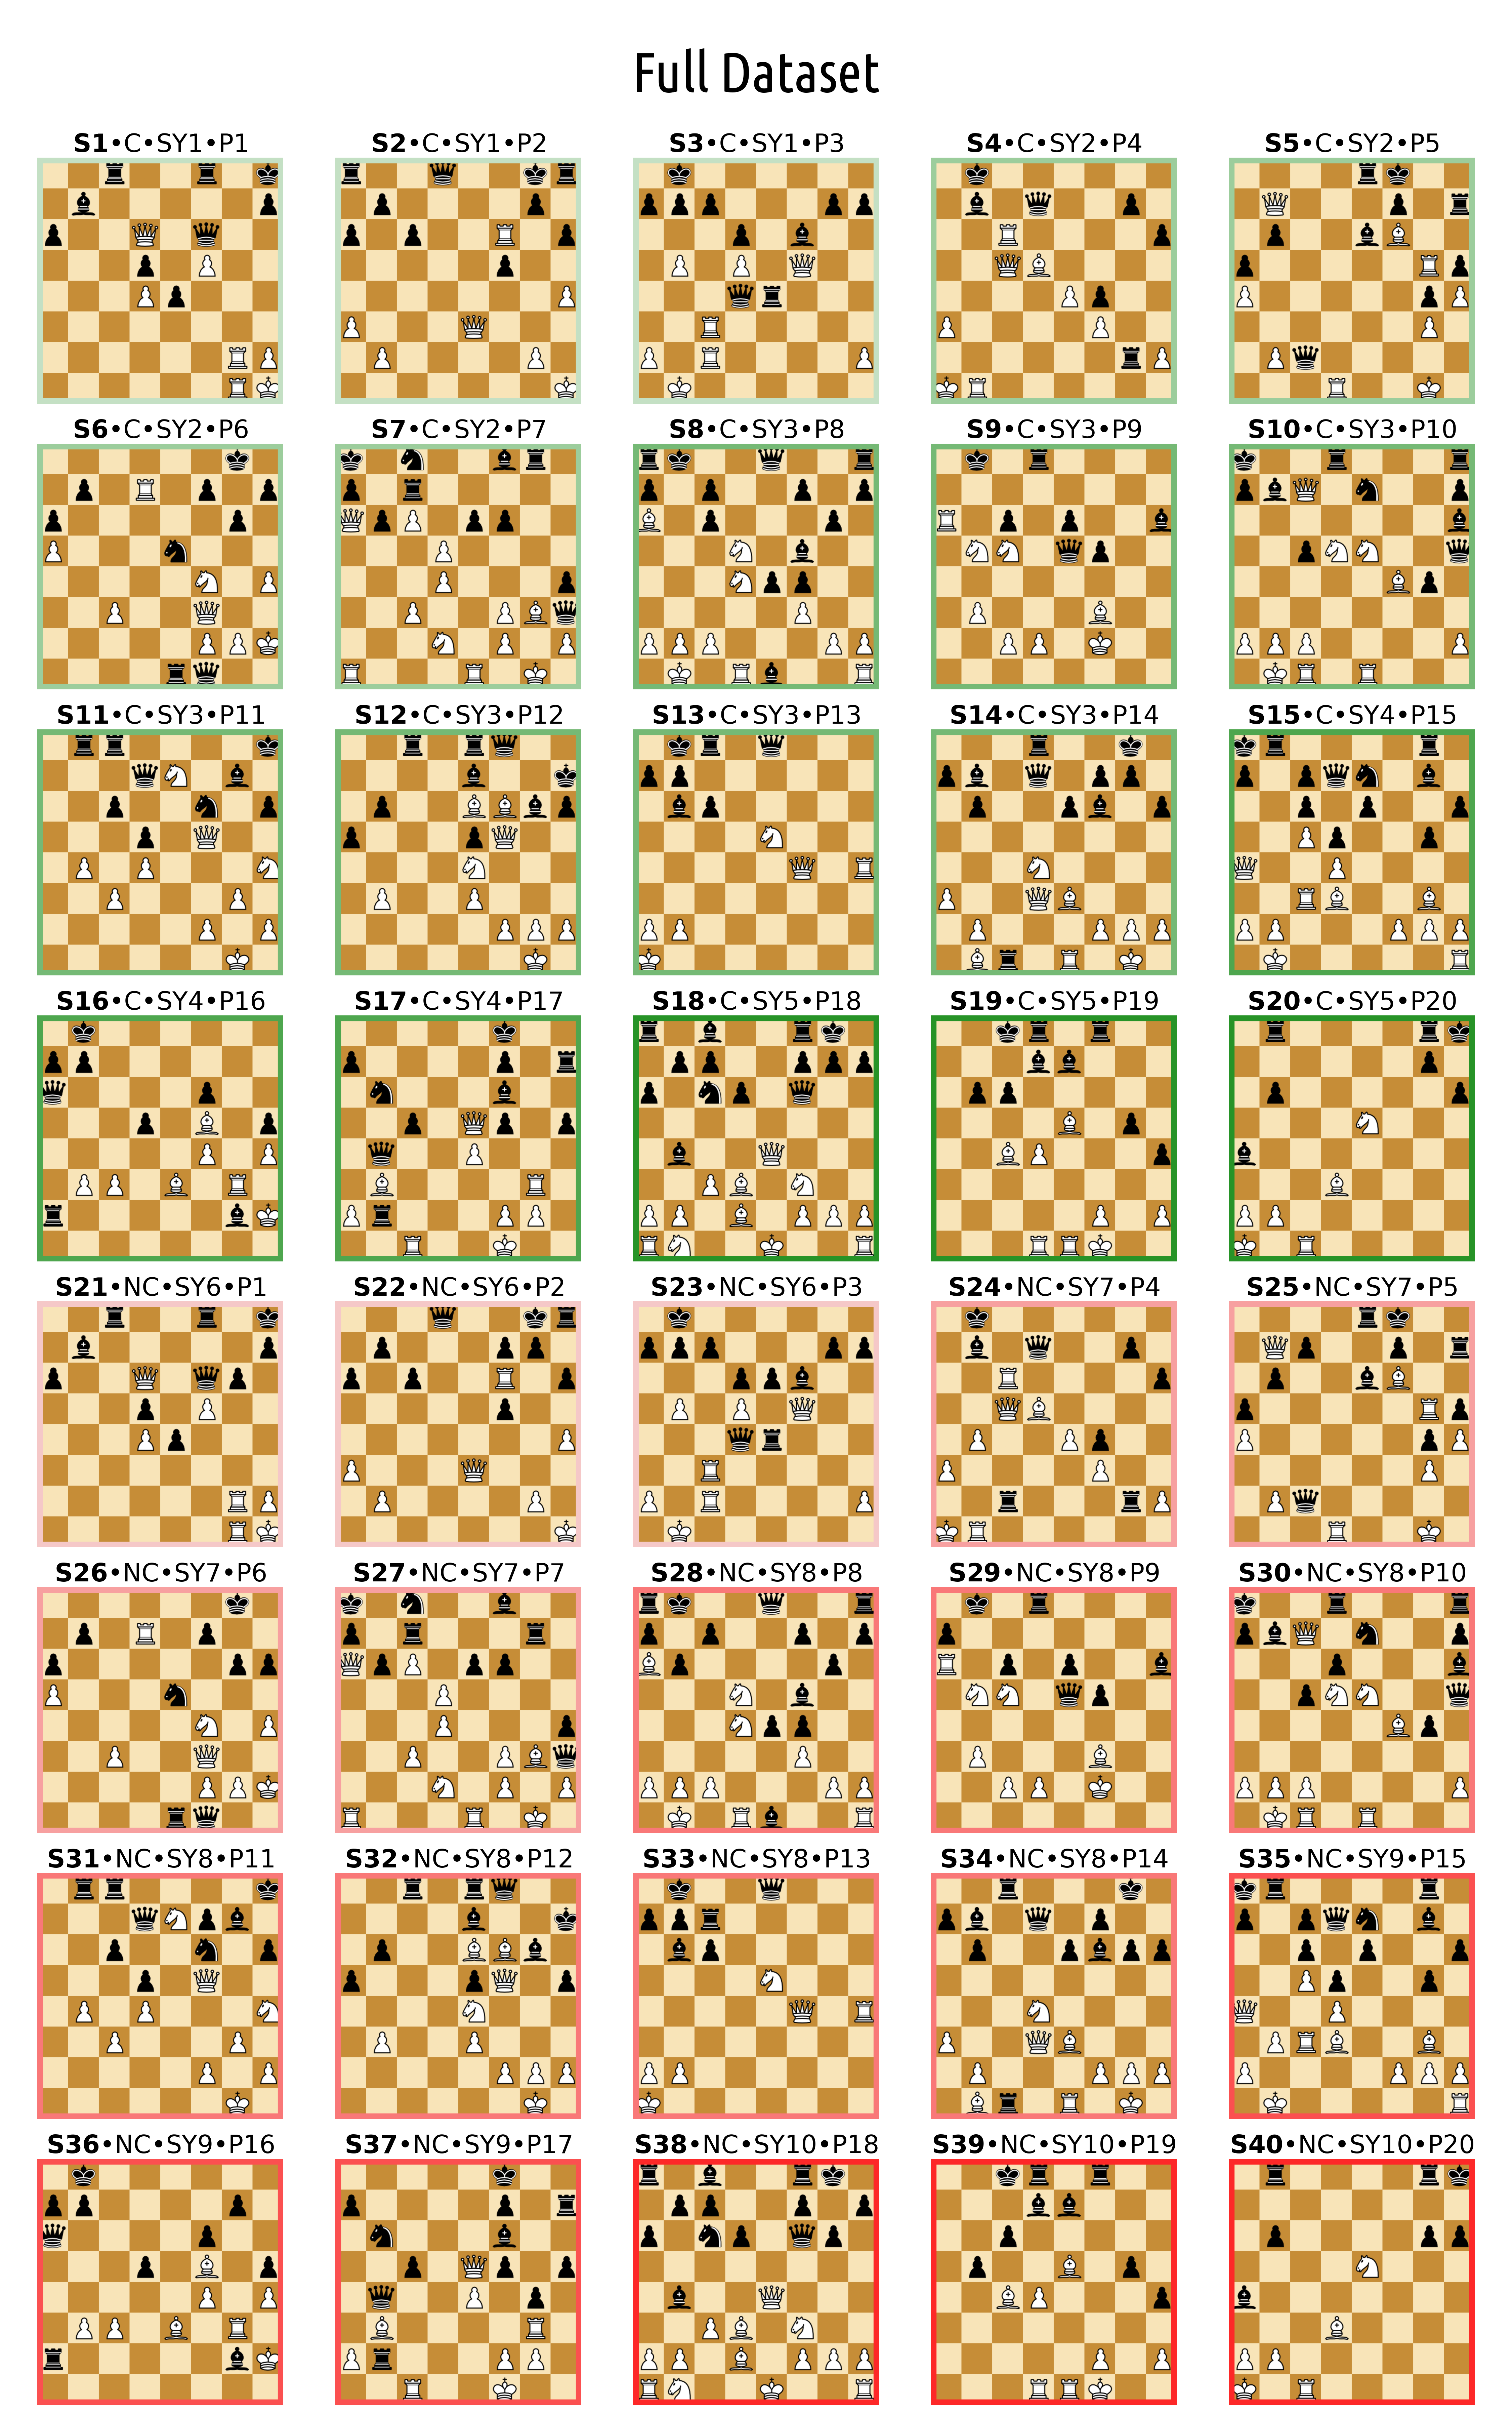
\includegraphics[width=0.8\linewidth]{write/figures/stimuli_with_tags.png}
  \caption{\textbf{Full stimulus set used in the experiment.} Each chessboard represents a unique stimulus from the dataset. The label above each board encodes: \textbf{S} (stimulus number), \textbf{C} or \textbf{NC} for checkmate and non-checkmate respectively, \textbf{SY} (strategy index), and \textbf{P} (visual pair). Borders are shaded: green tones for checkmate boards, red tones for non-checkmates. The hue intensity corresponds to the underlying strategy type.}
  \label{suppfig:all_stims}
\end{figure}

\supplementarysection{Stimulus Set Details}\label{suppsec:all_stims}

This supplementary section provides a comprehensive overview of the 40 chessboard stimuli used in the experiment, each labeled and visualized in Supplementary Fig.~\ref{suppfig:all_stims} and reported in Supplementary Table~\ref{supptab:stim_fens}. Stimuli were constructed to systematically vary along three key dimensions: whether they depicted an imminent checkmate (Checkmate vs.\ Non-checkmate), the tactical strategy leading to the checkmate (Strategy Type), and perceptual similarity (Visual Pairing). 

\emph{Checkmate} boards (C/NC) depicted configurations in which a forced mate sequence for White against Black existed, resolvable in four or fewer moves. Each checkmate board (denoted ``C'' in the figure) was paired with a non-checkmate counterpart (``NC'') that preserved the overall structure and piece configuration but introduced a minimal intervention—typically the repositioning of a single pawn—to neutralize the mating sequence while maintaining close visual similarity.

\emph{Strategy types} (SY) were defined according to both piece involvement and underlying tactical features, reflecting qualitative distinctions in how mating sequences are structured. These include queen–rook combinations (SY1 and SY6), involving coordinated linear tactics; supported attacks with minor pieces (SY2 and SY7), where auxiliary knights or bishops play a crucial role in sustaining the queen mate; minor piece mating nets (SY3 and SY8), relying on spatial confinement by knights and bishops; bishop-driven forcing moves (SY4 and SY9), emphasizing long-range control; and one-move checkmates (SY5 and SY10), which require minimal calculation and serve as structurally simple baselines.

\emph{Visual pairing} (P) designates stimuli matched primarily for perceptual similarity while holding relational structure constant. For each position, we also recorded the total number of pieces, the count of legal moves, the side of the board occupied by the defending king (left = 0, right = 1), and the dominant tactical motif characterizing the checkmate sequence. Where applicable, the number of moves required to reach checkmate is also noted.

\supplementarysection{fMRI data pre-processing}\label{suppsec:fmri-preproc}
\textbf{Anatomical data preprocessing} 
A total of 1 T1-weighted (T1w) images was found within the input BIDS dataset per subject. The T1w image was corrected for intensity non-uniformity (INU) with \texttt{N4BiasFieldCorrection} \cite{n4}, distributed with ANTs 2.5.1 \cite[RRID:SCR\_004757]{ants}, and used as T1w-reference throughout the workflow. The T1w-reference was then skull-stripped with a \emph{Nipype} implementation of the \texttt{antsBrainExtraction.sh} workflow (from ANTs), using OASIS30ANTs as target template. Brain tissue segmentation of cerebrospinal fluid (CSF), white-matter (WM) and gray-matter (GM) was performed on the brain-extracted T1w using \texttt{fast} \cite{fsl_fast} (RRID:SCR\_002823). Brain surfaces were reconstructed using \texttt{recon-all} \cite[FreeSurfer 7.3.2, RRID:SCR\_001847,][]{fs_reconall}, and the brain mask estimated previously was refined with a custom variation of the method to reconcile ANTs-derived and FreeSurfer-derived segmentations of the cortical gray-matter of Mindboggle \cite[RRID:SCR\_002438,][]{mindboggle}. Volume-based spatial normalization to one standard space (MNI152NLin2009cAsym) was performed through nonlinear registration with \texttt{antsRegistration} (ANTs 2.5.1), using brain-extracted versions of both T1w reference and the T1w template. The following template was selected for spatial normalization and accessed with \emph{TemplateFlow}
\cite[24.2.0,][]{templateflow}: \emph{ICBM 152 Nonlinear Asymmetrical template version 2009c} \cite{mni152nlin2009casym} (RRID:SCR\_008796; TemplateFlow ID: \texttt{MNI152NLin2009cAsym}).

\textbf{Functional data preprocessing}
For each of the BOLD runs found per subject, the following preprocessing was performed. First, a reference volume was generated, using a custom methodology of \emph{fMRIPrep}, for use in head motion correction. Head-motion parameters with respect to the BOLD reference (transformation matrices, and six corresponding rotation and translation parameters) are estimated before any spatiotemporal filtering using \texttt{mcflirt} \cite{mcflirt}. The BOLD reference was then co-registered to the T1w reference using \texttt{bbregister} (FreeSurfer) which implements boundary-based registration \cite{bbr}. Co-registration was configured with six degrees of freedom. Several confounding time-series were calculated based on the \emph{preprocessed BOLD}: framewise displacement (FD), DVARS and three region-wise global signals. FD was computed using two formulations following Power (absolute sum of relative motions, \cite{power_fd_dvars}) and Jenkinson (relative root mean square displacement between affines, \cite{mcflirt}). FD and DVARS are calculated for each functional run, both using their implementations in \emph{Nipype} following the definitions by \cite{power_fd_dvars}. The three global signals are extracted within the CSF, the WM, and the whole-brain masks. Additionally, a set of physiological regressors were extracted to allow for component-based noise correction \emph{CompCor} \cite{compcor}. Principal components are estimated after high-pass filtering the \emph{preprocessed BOLD} time-series (using a discrete cosine filter with 128s cut-off) for the two \emph{CompCor} variants: temporal (tCompCor) and anatomical (aCompCor). tCompCor components are then calculated from the top 2\% variable voxels within the brain mask. For aCompCor, three probabilistic masks (CSF, WM and combined CSF+WM) are generated in anatomical space. The implementation differs from that of Behzadi et al.~in that instead of eroding the masks by 2 pixels on BOLD space, a mask of pixels that likely contain a volume fraction of GM is subtracted from the aCompCor masks. This mask is obtained by dilating a GM mask extracted from the FreeSurfer's \emph{aseg} segmentation, and it ensures components are not extracted from voxels containing a minimal fraction of GM. Finally, these masks are resampled into BOLD space and binarized by thresholding at 0.99 (as in the original implementation). Components are also calculated separately within the WM and CSF masks. For each CompCor decomposition, the \emph{k} components with the largest singular values are retained, such that the retained components' time series are sufficient to explain 50 percent of variance across the nuisance mask (CSF, WM, combined, or temporal). The remaining components are dropped from consideration. The head-motion estimates calculated in the correction step were also placed within the corresponding confounds file. The confound time series derived from head motion estimates and global signals were expanded with the inclusion of temporal derivatives and quadratic terms for each \cite{confounds_satterthwaite_2013}. Frames that exceeded a threshold of 0.5 mm FD or 1.5 standardized DVARS were annotated as motion outliers. Additional nuisance timeseries are calculated by means of principal components analysis of the signal found within a thin band (\emph{crown}) of voxels around the edge of the brain, as proposed by \cite{patriat_improved_2017}. The BOLD time-series were resampled onto the following surfaces (FreeSurfer reconstruction nomenclature): \emph{fsnative}. All resamplings were performed with \emph{a single interpolation step} by composing all the pertinent transformations (i.e.~head-motion transform matrices, susceptibility distortion correction when available, and co-registrations to anatomical and output spaces). Gridded (volumetric) resamplings were performed using \texttt{nitransforms}, configured with cubic B-spline interpolation. Non-gridded (surface) resamplings were performed using \texttt{mri\_vol2surf} (FreeSurfer).

Many internal operations of \emph{fMRIPrep} use \emph{Nilearn} 0.10.4 \cite{nilearn} (RRID:SCR\_001362) , mostly within the functional processing workflow. For more details of the pipeline, see \href{https://fmriprep.readthedocs.io/en/latest/workflows.html}{the section corresponding to workflows in \emph{fMRIPrep}'s documentation}. 

\supplementarysection{Split-half Reliability of Behavioral RDMs}\label{suppsec:splithalf_bh_rdm}

To assess the reliability of behavioral Representational Dissimilarity Matrices (RDMs) in Experts and Novices, we computed split-half correlations using a permutation-based approach. For each group (Experts and Novices), we randomly split participants into two non-overlapping halves and compute separate RDMs with the same method as described in Sec.~\ref{sec:bh_rsa_section}. Spearman correlations were then computed between the lower triangles of the two RDMs. This procedure was repeated across 1,000 random permutations, yielding a distribution of split-half correlation coefficients for each group.

To test whether these reliability estimates were significantly greater than zero, we conducted one-sample \textit{t}-tests across the 1,000 permutations for each group. Additionally, we computed split-half correlations \textit{between} groups by comparing random halves of Experts to random halves of Novices, also across 1,000 permutations. Independent-samples \textit{t}-tests were used to compare Experts and Novices on both within- and between-group reliability scores. All statistical tests were two-tailed. All results are reported in Supplementary Table~\ref{supptab:bh_splithalf}.

We found that behavioral RDM reliability was higher in Experts: the mean split-half Spearman correlation \emph{within} the expert group was $r = 0.104$, while Novices showed $r = 0.030$. Split-half correlations \emph{between} Experts and Novices were negative (mean $r = -0.013$), indicating low cross-group similarity. These patterns suggest that expertise is associated with a more stable and shared representational geometry of the task domain: Experts exhibit more consistent pairwise dissimilarity structure across individuals, whereas Novices show weaker and more idiosyncratic structure; the near-zero difference in cross-group correlations ($\Delta r \approx 0$) further implies that expert and novice representations are organized differently rather than reflecting a simple strengthening of a common layout.

\begin{figure}[!htp]
  \centering
  \includegraphics[width=1\linewidth]{write/figures/roi_analysis_univ.png}
  \caption{\textbf{Univariate ROI differences (Experts vs. Novices).} Cortical parcels from the 180-area Glasser atlas showing group differences in second-level GLM contrast maps (\emph{Checkmate} $>$ \emph{Non-checkmate}, \emph{All} $>$ \emph{Rest}). Colors indicate the direction and relative magnitude of the Experts$-$Novices difference in contrast values. Maps are derived from the univariate analyses in Sec.~\ref{sec:fmri_glm}.}
  \label{suppfig:roi_analysis_univ}
\end{figure}

\begin{figure}[!htp]
  \centering
  \includegraphics[width=1\linewidth]{write/figures/roi_analysis_rsa.png}
  \caption{\textbf{ROI summaries of searchlight RSA group differences.} For each model RDM (Checkmate, Strategy, Visual similarity), whole-brain searchlight RSA maps were averaged within Glasser ROIs to compare Experts and Novices. \emph{Left}: uncorrected visualization. \emph{Right}: parcels surviving multiple-comparisons correction. Colors indicate the direction and relative magnitude of the Experts$-$Novices difference in model–brain correspondence. Maps are derived from the RSA analyses in Sec.~\ref{sec:fmri_rsa}.}
  \label{suppfig:roi_analysis_rsa}
\end{figure}

\supplementarysection{ROI analysis from uni and multivariate brain maps}\label{suppsec:roi_analysis}

To identify finer-grained anatomical regions showing significant differences in mean activation between Experts and Novices, we performed an exploratory second-level ROI analysis using the 180-region version of the Glasser parcellation described in Sec.~\ref{sec:rois}. We conducted this analysis on two sets of brain maps: the univariate first-level GLM contrast maps (Sec.~\ref{sec:fmri_glm}), and the searchlight RSA maps from Sec.~\ref{sec:fmri_rsa}. 

To facilitate anatomical interpretation, each ROI was additionally assigned a secondary label from the Harvard–Oxford cortical atlas. This was done by computing the center of mass of each ROI in MNI space and mapping the resulting coordinate to the nearest non-zero voxel in the 2\,mm Harvard–Oxford atlas (thresholded at 25\%). This combined approach allowed us to combine the spatial specificity of the Glasser atlas, which allows for more precise estimates of local activation patterns, with the broader and more familiar anatomical nomenclature of the Harvard-Oxford atlas.

\emph{Univariate contrast maps}
For each participant and contrast (\emph{Checkmate $>$ Non-checkmate}, \emph{All $>$ Rest}), we imported the first-level contrast images and extracted mean signal values from each of the 180 cortical ROIs using the \texttt{NiftiLabelsMasker} implementation in \texttt{nilearn}. This yielded a single scalar value per ROI per participant, resulting in group-level matrices for Experts and Novices that were used for statistical comparison. For each ROI, we performed an independent-samples $t$-test comparing Experts and Novices, and computed the mean group difference, $t$-statistic, FDR-corrected $p$-value, and the 95\% confidence interval of the difference. Results for significant ROIs are reported in Supplementary Table~\ref{supptab:roi_analysis_univ_allrest} and visualized in Supplementary Figure \ref{suppfig:roi_analysis_univ}.

Univariate analyses were suggestive of several activation spots at or near locations that have been previously investigated in expertise literature, but in many cases these differences did not survive correction for multiple comparisons. This strengthens the suspicion that was the major motivation for our study: namely, that the classic univariate approach is not sensitive to the many ways in which expertise changes neural processing.

\emph{RSA searchlight maps}
To facilitate anatomical interpretation of the searchlight RSA results, and to complement the univariate group-level analysis with a "content-oriented" approach, we applied the same second-level ROI-based procedure described in the above paragraph. For each participant theoretical model (Checkmate, Strategy, Visual Similarity), we imported the individual whole-brain correlation maps obtained from the searchlight (see Sec.~\ref{sec:neurosynth_analysis}), extracted the mean correlation value within each of the 180 Glasser ROIs, and performed independent-samples $t$-tests comparing Experts and Novices ROI-wise. Anatomical labels from the Harvard–Oxford cortical atlas were assigned to each ROI based on their center of mass.

Results from this analysis (see Supplementary Tables~\ref{supptab:roi_analysis_rsa_check} and \ref{supptab:roi_analysis_rsa_strategy}, and Supplementary Figure \ref{suppfig:roi_analysis_rsa}) showed more extensive networks involved in chess expertise than the univariate counterpart. On the one hand, this suggests that multi-variate approaches may tap onto complementary aspects than univariate ones, and on the other that expertise effects in the brain may involve broader networks than previously thought.

\begin{figure}[!htp]
  \centering
  \includegraphics[width=1\linewidth]{write/figures/rsa_vs_decoding_main.png}
    \caption{\textbf{Comparison of RSA and decoding on the main model dimensions.} ROI-wise summaries of model–brain correspondence (RSA) versus linear classification accuracy (SVM decoding) for the three primary dimensions (Checkmate, Strategy, Visual similarity). Panels juxtapose RSA (left) and decoding (right) to highlight convergences and divergences across the 22 Glasser ROIs. Colors indicate ROI groups; asterisks indicate significant regions (Experts $>$ Novices) after FDR correction.}
      \label{suppfig:rsa_vs_decoding_main}
\end{figure}

\begin{figure}[!htp]
  \centering
  \includegraphics[width=1\linewidth]{write/figures/rsa_vs_decoding.png}
    \caption{\textbf{Comparison of RSA and decoding on finer dimensions (checkmate stimuli only).} As in Fig.~\ref{suppfig:rsa_vs_decoding_main}, but restricted to checkmate boards and extended to finer categorizations (Strategy within checkmates, Motif, Total pieces, Legal moves, and White moves to mate). RDMs derived from the finer dimensions are shown in the central panel. Colors indicate ROI groups; asterisks indicate significant regions (Experts $>$ Novices) after FDR correction.}
      \label{suppfig:rsa_vs_decoding_finer}
\end{figure}

\supplementarysection{Brain Decoding}\label{suppsec:brain-decoding}
% Purpose and rationale
To assess whether local voxel patterns encoded linearly decodable information about chess-relevant categories, we conducted multivariate classification analyses using support vector machines (SVMs). These analyses evaluated the discriminability of activation patterns across different conditions within each region of interest (ROI), providing a functional readout of category-selective information.

% Input data and ROI setup
Classification analyses were implemented in MATLAB R2024b using the CoSMoMVPA toolbox \cite{oosterhof2016cosmomvpa}. As explained in Sec.~\ref{sec:fmri_glm}), we used the unsmoothed beta estimates of the 40 conditions as the input of these analyses. For each subject and run, multi-voxel patterns were extracted from predefined ROIs, including bilateral cortical mask from the Glasser atlas~\cite{glasser2016multi} (See section \ref{sec:rois} for more details). All analyses were performed separately for each ROI and participant.

% SVM training, partitioning, and targets
For each ROI, a linear SVM classifier (\texttt{@cosmo\_classify\_svm}) was trained to discriminate between condition labels derived from the experimental design. Classification targets were constructed from categorical regressors (e.g., Checkmate, Strategy, Visual similarity). The data were partitioned using an $n$-fold cross-validation scheme across runs (leave-one-run-out), with balanced folds ensured via \texttt{cosmo\_balance\_partitions}. Within each fold, voxel patterns were labeled with their corresponding class and used to train and test the classifier.

% Accuracy computation and filtering
Decoding accuracy was defined as the mean classification performance across cross-validation folds. ROIs with fewer than 10 usable voxels were excluded to ensure minimum feature dimensionality. Accuracy scores were computed independently for each participant, regressor, and ROI.

% Intro and visual similarity (no robust results)
Supplementary Table~\ref{tab:svm_roi_summary} and Supplementary Fig.~\ref{suppfig:rsa_vs_decoding_main} reports SVM decoding accuracy across ROIs for each main model dimension. Decoding based on the \emph{Visual Similarity} model yielded restricted but significant effects. While some ROIs showed above-chance classification (e.g., posterior cingulate: $M = 0.028$; superior parietal: $M = 0.028$), the majority of visual and high-level areas did not exhibit significant decoding for this perceptual dimension. Decoding accuracy in early and primary visual cortex was low and non-significant (e.g., early visual: $M = -0.040$), suggesting that visual similarity alone did not strongly shape the separability of neural patterns in these regions.

% Strategy decoding: broad, robust, parietal-frontal + dorsal stream
In contrast, decoding of the \emph{Strategy} dimension revealed robust group-level accuracy across a broad network of ROIs. Experts showed reliable above-chance decoding in the superior parietal lobule ($M = 0.046$), inferior parietal lobule ($M = 0.035$), and dorso-lateral prefrontal cortex ($M = 0.027$). Additional significant decoding was observed in premotor cortex ($M = 0.033$), paracentral lobule and mid-cingulate ($M = 0.024$), and insular and frontal opercular cortex ($M = 0.013$). Effects also extended to dorsal stream visual areas ($M = 0.018$), highlighting their role in abstract relational processing. These findings indicate that expert representations are sufficiently structured along strategy-related dimensions to permit reliable linear classification.

% Checkmate decoding: similar pattern, high-level areas
Decoding of \emph{Checkmate vs. Non-checkmate} boards yielded a similar spatial profile. High classification accuracy was observed in dorso-lateral prefrontal cortex ($M = 0.080$), inferior parietal cortex ($M = 0.089$), and superior parietal cortex ($M = 0.053$). Additional significant effects were found in lateral temporal cortex ($M = 0.052$), premotor areas ($M = 0.052$), and posterior cingulate cortex ($M = 0.035$), indicating that goal-related distinctions such as checkmate status were reliably encoded in higher-order associative cortices.

% Finer decoding
Aside our main decoding analysis (i.e., on the three main dimension built into our dataset), we also performed a finer decoding analysis on five additional possible categorizations of the checkmate boards. This finer analysis allow us to assess what information can be decoded within the checkmate class, offering a proxy into how strategic information may be structured. Specifically, we performed a decoding analysis on: Strategy (the same as in the main analysis, but now using only the 20 checkmate chess boards), Motif, Total number of pieces, Total number of available legal moves, and Number of white moves to checkmate. All the results for this analysis (and their RSA counterparts) are reported in Supplementary Tables~\ref{tab:svm_roi_summary_checkonly} and~\ref{tab:rsa_roi_summary_checkonly}, and visualized in Supplementary Fig.~\ref{suppfig:rsa_vs_decoding_finer}.

\begin{figure}[!htp]
  \centering
  \includegraphics[width=1\linewidth]{write/figures/rdm_intercorr.png}
    \caption{\textbf{Orthogonality of representational dissimilarity matrices.} 
    \textbf{Top row:} Bar plots showing the Spearman correlation between each target RDM and the other two predictors, both as pairwise correlations and partial correlations (controlling for the third RDM). Each bar reflects the strength of association ($\rho$), with partial correlations labeled as ``(partial X)'' to indicate the variable that was controlled for. 
    \textbf{Bottom row:} Variance partitioning results for each target RDM. Bars indicate the proportion of variance uniquely explained by each predictor RDM, variance shared between predictors, and residual (unexplained) variance. Larger unique and smaller shared contributions suggest greater orthogonality among representational structures.}
      \label{suppfig:rdm_orthogonality}
\end{figure}

\supplementarysection{Orthogonality Across RDMs}

To quantify the degree of overlap and separability among representational structures in our dataset, we first computed pairwise Spearman correlations between the flattened upper triangle of each model RDM (excluding the diagonal), providing a measure of shared variance in representational structure. We then computed partial Spearman correlations, which estimate the relationship between two RDMs while controlling for variance explained by the third. For instance, the partial correlation between the Checkmate and Strategy RDMs, controlling for Visual Similarity, reflects their unique association independent of the shared structure with the Visual RDM. 

To further disentangle representational overlap, we further conducted a variance partitioning analysis based on nested linear regression models. Each RDM was treated in turn as a dependent variable, with the remaining two serving as predictors. We fit a full multiple linear model using both predictors to explain variance in the target RDM, and two reduced models each omitting one predictor. The unique variance explained by each predictor was calculated as the difference in $R^2$ between the full model and the corresponding reduced model. Shared variance was defined as the portion of $R^2$ explained by both predictors jointly, beyond their individual contributions, and residual variance captured the unexplained portion.
Formally, given a target RDM $Y$ and two predictors $X_1$ and $X_2$, we define:
\[
\begin{aligned}
R^2_{\text{full}} &= R^2(Y \sim X_1 + X_2) \\
R^2_{\text{reduced}_1} &= R^2(Y \sim X_2) \\
R^2_{\text{reduced}_2} &= R^2(Y \sim X_1) \\
\text{Unique}_{X_1} &= R^2_{\text{full}} - R^2_{\text{reduced}_1} \\
\text{Unique}_{X_2} &= R^2_{\text{full}} - R^2_{\text{reduced}_2} \\
\text{Shared} &= R^2_{\text{full}} - \text{Unique}_{X_1} - \text{Unique}_{X_2} \\
\text{Residual} &= 1 - R^2_{\text{full}}
\end{aligned}
\]
Any negative values arising from this decomposition due to noise or multicollinearity were set to zero for interpretability. This approach provides a formal quantification of the unique and shared variance attributable to each representational model, allowing us to assess the degree of orthogonality between theoretical representational geometries.

The variance partitioning analysis revealed that the three RDMs are well-separated and largely independent (see~\ref{suppfig:rdm_orthogonality}, with each predictor explaining predominantly unique rather than shared variance. This orthogonality validates the theoretical distinctiveness of the representational structures captured by the \textit{Check}, \textit{Strategy}, and \textit{Visual} RDMs, indicating that they reflect genuinely different aspects of chess board representation. The predominance of unique variance over shared variance supports the use of these RDMs as independent predictors in subsequent analyses, as they capture complementary rather than redundant information about stimulus similarity structure.

\begin{figure}[!htp]
 \centering
 \includegraphics[width=0.6\linewidth]{write/figures/eyetrack.png}
   \caption{\textbf{Decoding chess expertise from eye-tracking data.} Each dot represents the cross-validated accuracy from one of the $k=20$ stratified group folds. \textbf{Left:} decoding based on two-dimensional gaze coordinates (x, y). \textbf{Right:} decoding based on displacement from screen center. The solid horizontal line shows the mean accuracy across folds; the dashed line indicates chance level (0.5). The shaded band marks the 95\% confidence interval around the mean, computed using the Student's $t$-distribution.}
 \label{suppfig:eyetrack_results}
\end{figure}

\supplementarysection{Groups cannot be inferred from estimated eye-movements}

To investigate whether estimated eye-movement patterns differ systematically between chess Experts and Novices, we performed two separate decoding analyses using support vector machines (SVM). The first analysis used the estimated gaze coordinates (x, y), while the second used the corresponding displacements from the center of the screen. These estimates were derived from functional MRI data using BidsMReye (\href{https://github.com/cpp-lln-lab/bidsMReye}), a BIDS-ready version of DeepMReye~\cite{frey2021magnetic}.

We included the full sample of 40 participants (20 Experts and 20 Novices). For each participant, all available task runs were used; each run was treated as an independent sample. The input features for each sample were constructed by flattening the time series of the gaze coordinates or displacement values within a run, resulting in a subject-run-level feature vector. This yielded a feature matrix $X \in \mathbb{R}^{n \times d}$, where $n$ is the number of runs and $d$ is the number of timepoints times two (for x and y) or one (for displacement). Binary class labels $y \in \{0, 1\}^n$ indicated expertise (expert = 1, novice = 0), and subject identifiers were recorded to define cross-validation groups.

We assessed classification performance using stratified group $k$-fold cross-validation with $k = 20$ folds, as implemented in \texttt{StratifiedGroupKFold} from \texttt{scikit-learn}. This procedure ensured that samples from the same participant were never split between training and test sets (i.e., we used 19 subjects per group as training set and one subject per group as test set). Folds were stratified by class to preserve expert/novice balance.

Within each fold, we trained a support vector classifier with a linear kernel using a pipeline that included z-scoring of input features via \texttt{StandardScaler}. The model was trained on all runs from all training participants and evaluated on the runs from the held-out participants. For each test sample, we recorded the predicted class label and the posterior probability (decision function output) for being classified as an expert. This process was repeated for all folds, and the predicted labels and probabilities were aggregated across folds.

Performance was quantified using overall accuracy, balanced accuracy, and F1-score. To statistically assess whether decoding exceeded chance, we performed a one-sample $t$-test on the distribution of fold-wise accuracies against a null hypothesis of 0.5 (chance), and computed the binomial probability of the number of correctly classified runs under chance performance. Results are reported in Supplementary Fig. \ref{suppfig:eyetrack_results} and Supplementary Table \ref{supptab:et_decoding_results}.

\begin{figure}[!ht]
    \centering
    \includegraphics[width=1\linewidth]{write/figures/pr_supp.png}
    \caption{\textbf{Relationship between PR and ROI size} (number of voxels), plotted separately for Experts (left), Novices (center), and group differences (right). Each dot represents one ROI; lines indicate linear regression fits, with corresponding Pearson correlation coefficients. These analyses test whether PR scales with anatomical extent and whether this relationship differs between groups.
  }
    \label{suppfig:pr_suppl}
\end{figure}

\supplementarysection{Participation ratio is not predicted by ROI size}

To assess how regional dimensionality relates to anatomical size, we computed the participation ratio (PR) within each cortical ROI for each participant. We then averaged PR values across participants within each group (Experts and Non-Experts) and calculated the difference (Expert minus Non-Expert) per ROI. Finally, we visualized and quantified the relationship between PR and ROI size by plotting these measures against each other and computing Pearson correlation coefficients (see Fig.~\ref{suppfig:pr_suppl}).

\begin{figure}[!htp]
    \centering
    \includegraphics[width=.8\linewidth]{write/figures/terms_flat.png}
    \caption{\textbf{Neurosynth meta-analytic cognitive maps.} The maps are showed in volume space along with the corresponding surface projection.}
    \label{suppfig:flat_terms}
\end{figure}

\clearpage

\input{write/tables/stimuli}
\input{write/tables/bh_rdm_splithalf}
\input{write/tables/rsa_main_dims}
\input{write/tables/decoding_main_dims}
\input{write/tables/mvpa_extended_dimensions}
\input{write/tables/pr_ttest}
\input{write/tables/neurosynth_rsa}
\input{write/tables/neurosynth_univ}
\input{write/tables/roi_maps_rsa} 
\input{write/tables/roi_maps_univ} 
\input{write/tables/et_decoding}



\end{document}